\documentclass{Vorlage}
%\usepackage[ngerman]{babel}
\usepackage{amsfonts}
\usepackage{graphicx}
\usepackage{url}
\usepackage{amsmath}
\usepackage{adjustbox}
\usepackage{color}
\usepackage{multirow}
\usepackage{bm}
\usepackage{cite}
\usepackage{subfigure}
%\usepackage[utf8]{inputenc}
%\bibliographystyle{apalike}
\setlength{\parindent}{0pt}
\usepackage{tabularx}

\pagestyle{fancy}
\renewcommand*\sectionmark[1]{\markboth{\MakeUppercase{#1}}{}}
\begin{document}

\newgeometry{top=2.5cm,bottom=2.0cm,left=2.5cm,right=2.5cm} % Befehl wird nur benötigt, falls Änderungen an den Seitenrändern in der Datei "Vorlage.cls" vorgenommen werden.

\begin{titlepage}

\begin{figure}
 \begin{center}
 
\includegraphics[scale=0.8]{Pictures/logo3}
 \end{center}
\end{figure}
\vspace*{3cm}




\titel{Kleinräumige Extrapolation von Umfragedaten}{}

\vspace{1cm}

\begin{tabular}{p{3.5cm}|p{0.1cm} p{10cm}l}
\textsc{Namen:} & & \textsc{Alexander Lange, Kai Husmann}\\
\textsc{Matr. Nr.:} & & \textsc{21426614, 20707176}\\
\textsc{Studiengang:} & & \textsc{Angewandte Statistik}\\
\textsc{Mail:} & & \textsc{Alexander.lange$ @ $uni-goettingen.de}\\
\textsc{} & & \textsc{Kai.Husmann$ @ $forst.uni-goettingen.de}\\
\textsc{Kurs:} & & \textsc{Statistisches Praktikum}\\
\textsc{Kursleiter:} & & \textsc{Prof.Dr. Thomas Kneib}\\
\textsc{Lehrstuhl:} & & \textsc{Statistik}\\
\textsc{Fakultät:} & & \textsc{Wirtschaftswissenschaften}\\
\textsc{Abgabedatum:} & & \textsc{30. September 2016}\\
\end{tabular}
\end{titlepage}

\restoregeometry

\pagenumbering{Roman} % \pagenumbering{roman} = Kleinschreibung: II -> ii.

\pagestyle{plain}

\tableofcontents % Inhaltsverzeichnis.

\newpage % Neue Seite.

\listoffigures % Abbildungsverzeichnis.

\newpage

\listoftables % Tabellenverzeichnis.

\newpage

\pagenumbering{arabic} % Ab hier folgt die arabische Seitennummerierung.

%\renewcommand{\thesection}{\arabic{section}} % Römische Nummerierung der Kapitelüberschriften.

%============================================ Instroduction ========================================================%
\pagestyle{fancy}

\section{Einleitung}
Kleinräumige Extrapolation von Umfragedaten besitzt vor allem eine hohe Relevanz bei Städten, Kommunen und Gemeinden um städtische oder ländliche Planung auf wissenschaftlich fundierten Erkenntnissen voranzutreiben \cite{Planung}. Dabei kann die konkrete Fragestellung bzw. das Anwendungsgebiet sehr vielfältig sein. Es kann genutzt werden, um z.B. Landschaftsbilder nach den Vorstellungen und im Einvernehmen mit den Einwohnern einer Region zu Planen \cite{Natur}, oder um die Infrastruktur von Kommunen den Bedürfnissen der Bürger durch den demographischen Wandel anzupassen \cite{Lubeck}.\\
So werden auch in dieser Arbeit Regionale Daten genutzt, um spezifische Fragestellungen zu beantworten, die den Aufgaben einer städtischen Verwaltung korrespondieren. Konkret handelt es sich um Daten zur Bevölkerung Stuttgarts. Dabei stehen Stichproben Datensätze zur Verfügung die in etwa 0,05\% der Gesamtbevölkerung, also der Grundgesamtheit, Stuttgarts repräsentieren. Ziel dieser Arbeit ist es anhand von statistischen Methoden die Informationen der Stichprobe zu nutzen um nachfolgende Fragestellungen für die Grundgesamtheit Stuttgarts zu beantworten.\\
Es handelt sich zum einen um die Frage: Wie ist die Meinung zu Stuttgart 21? Zum anderen geht es um die Frage: Wie ist die Wohnzufriedenheit in Stuttgart?

Fragestellungen: Wie ist die Wohnzufriedenheit in Stuttgart? Wie ist die Meinung zu Stuttgart 21? Kleinräumige Extrapolation
Obwohl die Formulierung \textit{nicht-parametrisch} für den in dieser Arbeit verwendeten Spline-Typ mathematisch unpräzise ist \cite[p. 1]{eilers1996}, wird sie, wie in der Literatur üblich, synonym für \textit{semiparametrisch} verwendet.
Modllierung hat zwei Aussagen: 1. Parameterbeschriebung-Interpretation des Modells, 2. Extrapolation: Prognose
\newpage

%=================================================== Main Part  ====================================================%
\section{Material und Methoden}
\subsection{Daten}
Insgesamt liegen für die Analysen drei Umfragen mit unterschiedlichen Stichprobenumfängen vor. Die kleinste Datei 
enthält Angaben zur Bewertung der Wohngegend, der Meinung zu Stutttgart 21 sowie weitere sozioökonomische Kovariablen, 
die zur Erklärung der beiden abhängigen Variablen dienen sollen. Sie wird im Folgenden als 
Parametrisierungsstichprobe bezeichnet. Die Parametrisierungsumfrage ist eine Stichprobe von 
der die Grundgesamtheit im strikteren Sinne für eine Validierung nicht zur Verfügung steht. Alle Modellqualitätskriterien müssen 
demnach entweder an der Stichprobe selbst oder an einer anderen Erhebung entwickelt werden. Die beiden anderen 
Umfragen haben jeweils einen deutlich größeren Stichprobenumfang. An diesen Umfragen werden die parametrisierten 
Modelle angewendet und die Meinung zu Stuttgart 21 sowie die Wohnzufriedenheit somit kleinräumig extrapoliert. Einige 
Variablen unterscheiden sich in ihren Ausprägungen zwischen den Umfragen. Zur Vereinheitlichung der Dateien mussten 
einige Gruppenausprägungen demnach umkodiert werden. Die Umkodierungen können in der digital anhängenden Datei 
\textit{Aufbereitung\_Stuttgart21.R} nachvollzogen werden.

\subsubsection{Parametrisierungsstichprobe}
Mit den Datensätzen der Parametrisierungsstichprobe (Tabelle \ref{Datensatz}) werden die Modelle für die kleinräumige 
Extrapolation parametrisiert. Bei dieser Umfrage handelt es sich um eine Befragung aus dem Jahr 2015 zur Lebensqualität 
der Einwohner Stuttgarts bei der unter anderem die Bewertung der Wohnsituation und die Meinung zu Stuttgart 21 abgefragt 
wurden \cite{Stuttgart2015}. Insgesamt standen 8 sozioökonomische Variablen und Angaben zur räumlichen Lage zur 
Verfügung. Von jedem Datensatz waren die stetige räumliche Lage als Gauß-Krüger Geokoordinate sowie die diskrete räumliche 
Lage im Stadtteil und Stadtbezirk bekannt.\\

\begin{table}[h]
\centering
\caption{Erhobene sozioökonomische und geographische Variablen der Parameterisierungsstichprobe und deren Anzahl der Ausprägungen sowie vermutete Modellierung im additiven Modell.}
\label{Datensatz}
\adjustbox{max height=\dimexpr\textheight-5.5cm\relax,
           max width=\textwidth}{
\begin{tabular}{l|c|c}
\multicolumn{2}{l}{Anzahl Beobachtungen: 3.143}     \\ \hline \hline
\textbf{Variable} & \textbf{Anzahl Ausprägungen} & \textbf{Modellierung} \\ \hline
Bewertung Wohngegend &  6 & Geordnet Kategorial \\ \hline
Meinung Stuttgart 21 &  6 & Geordnet Kategorial \\ \hline
Personenanzahl im Haushalt & 5 & Nicht Parametrisch \\ \hline
Monatliches Netto Haushaltseinkommen & 6 & Nicht Parametrisch \\ \hline
Altersklasse Befragter & 6 & Nicht Parametrisch \\ \hline
Geschlecht & 2 & Parametrisch\\ \hline
Familienstand & 4 & Parametrisch \\ \hline
Nationalität & 2 & Parametrisch \\ \hline
Stadtbezirk & 23 & Markov-Zufallsfeld \\ \hline 
Stadtteil &  142 & Markov-Zufallsfeld \\ \hline 
Gauß-Krüger & & Tensorprodukt-Splines  \\ \hline \hline
\end{tabular}
}
\end{table}


In Tabelle \ref{Datensatz} sind nicht nur die Anzahlen der Ausprägungen der Variablen, sondern auch die vermuteten 
Formen der Einflüsse der Kovariablen auf die abhängigen Variablen nach visueller Einschätzung aufgelistet. Es ist 
ersichtlich, dass alle nominal skalierten Variablen, wie z.B. die Nationalität, als parametrisch und dass 
alle kardinal skalierte Variablen, wie z.B. die Altersklasse des Befragten, als nicht-parametrisch 
modelliert werden sollten. Laut \cite[p.9]{fahrmeir2009regression} sind diese beobachteten Zusammenhänge typisch für 
eine Regressionsanalyse. In Anlehnung an \cite[p. 503 ff. \& p. 524 ff.]{fahrmeir2013regression} wird der 
kontinuierliche räumliche Effekt durch ein Tensor Produkt und die diskreten räumlichen Effekte durch ein Markov-Zufallsfeld im additiven Regressionsmodell berücksichtigt.\\
Für die Auswahl der geeigneten Regressionsmethode und der Ergebnisinterpretation ist es hilfreich, das Verhältnis der 
Häufigkeiten der Kategorienausprägungen der abhängigen Variable zu kennen und seltene Ereignisse zu identifizieren. 
Während die meisten befragten Personen ihre Wohngegend mit \textit{gut} oder \textit{sehr gut} bewertet haben, treten 
Beobachtungen mit \textit{schlechter} oder \textit{sehr schlechter} Einschätzung relativ selten auf (Tabelle 
\ref{endogene}). Im Vergleich sind die Verhältnisse der Gruppenhäufigkeiten zur Meinung zu Stuttgart 21 
ausgeglichener. Die \textit{neutrale} Haltung ist etwa halb so häufig vertreten wie die \textit{zustimmende} Haltung. 
Bei beiden Variablen wurden die wenigen, für die Modellierung irrelevanten, Kategorien 
\textit{Keine Angabe} entfernt. Den Variablen kann in bei der Gruppenausprägung eine Rangfolge, jedoch kein 
Intervall unterstellt werden. Es handelt sich demnach in beiden Fällen um ordinal Skalierte Daten.

\begin{figure}[h]
 \begin{center}
 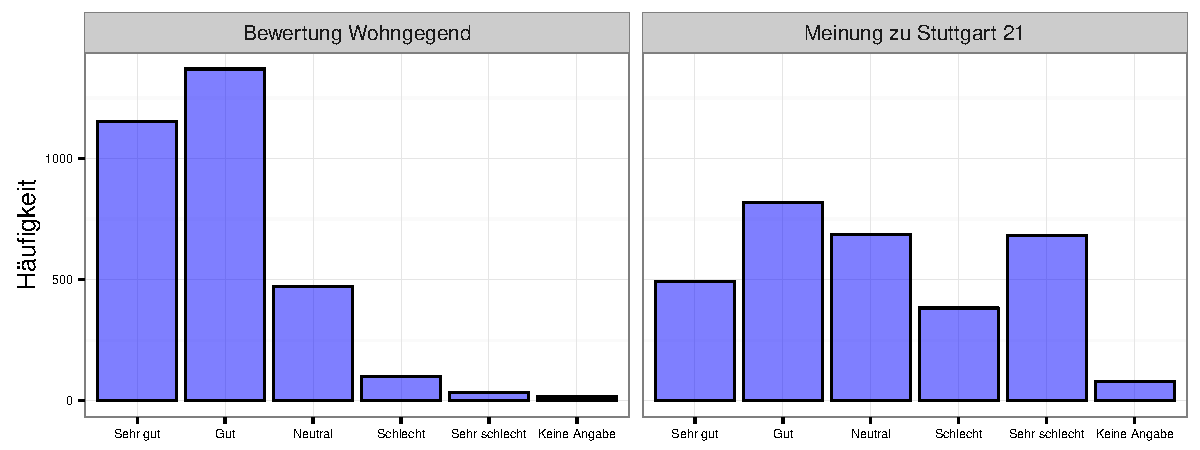
\includegraphics[scale=0.8]{Pictures/BarResp}
 \caption{Häufigkeit der Kategorienausprägungen der endogene Variablen in der Parameterisierungsstichprobe.}
 \label{endogene}
 \end{center}
\end{figure}

Das amtliche, nach Stadtteilen oder Stadtbezirken aufgelöste Ergebnis der Volksabstimmung zu Stuttgart 21 von 2011 kann 
dem Internetauftritt der Stadt entnommen werden \cite{Amt}. Es bietet sich dadurch eine zusätzliche Möglichkeit zur 
Modellevaluierung an, indem die Modellierungsergebnisse mit den tatsächlichen Ergebnissen verglichen werden. Da bei der 
Abstimmung mit Sicherheit nur die beiden Kategorien (\textit{Zustimmung} und \textit{Ablehnung }) unterschieden werden 
können, wurden die Gruppenausprägungen der Parameterisierungsstichprobe neu zusammengefasst. In den Rohdaten wurden noch 
6 Gruppen unterschieden. Es wurde eine Neugruppierung in drei Gruppenausprägungen vorgenommen (Tabelle \ref{endogene}). Dafür wurden jeweils die 
Gruppen \textit{sehr gut} und \textit{gut} zu \textit{Zustimmung} und \textit{schlecht} und \textit{sehr schlecht} zu 
\textit{Ablehnung} zusammengefasst. Falls nur \textit{Zustimmung} und \textit{Ablehnung} für die Modellierung 
berücksichtigt werden sollen, reduziert sich der Stichprobenumfang auf 2377 Beobachtungen. Dadurch bleibt die 
Möglichkeit erhalten eine multinomial verteilte abhängige Variable zu modellieren und trotzdem eine Validierung für 
zwei Klassen vorzunehmen. Für die exogen in die Analyse einfließenden Variablen sind detailliertere Informationen zu den 
Häufigkeiten der Ausprägungen im Anhang verfügbar (Abbildung \ref{exogen_parametrisierungsdatensatz}). 
\textcolor{red}{bei der abb. Einkommen müsste es $<900$ statt 900 sein}\\

Da in dieser Arbeit ein Schwerpunkt auf der Analyse unterschiedlicher räumlicher Effekte liegt, vergleicht dieser Abschnitt alle drei räumlichen Effekte in Bezug zu den beiden endogenen Variablen. Abbildung \ref{XYStuttgart3} zeigt die absolute Häufigkeit der Beobachtungen der Meinung zu Stuttgart 21 in kontinuierlicher räumlicher Lage. Zur besseren Übersicht wurden nicht alle Beobachtungen geplottet, sondern Beobachtungsdichten über bivariate normalverteilte Kerndichteschätzer mit festem Abstand für jede Richtungen ermittelt \cite{ggplot} sowie \cite{MASS}. Um die Hintergrundkarte einbinden zu können wurden die Gauß-Krüger Koordinaten in Dezimalgrad umgerechnet. Da absolute Dichten dargestellt werden, ist die Dichte der Kategorien nicht nur von der Anzahl der Kategorien selbst, sondern auch von der Einwohnerdichte beeinflusst. Des weiteren wird die Dichte von der Ausschöfung, also der Anzahl beantworteter Befragungsbögen beeinflusst. Wegen der hohen Einwohnerdichte im Innenstadtbereich sind dort die Beobachtungsdichten aller 3 Klassen tendenziell höher als in den Randbezirken. Des weiteren ersichtlich ist, dass einige Bereiche, wie das Naturschutzgebiet \textit{Rotwildpark} im Westen oder der \textit{Schurwald} im Osten, aufgrund ihrer geographischen Beschaffenheit oder Landnutzungsform nicht oder relativ dünn besiedelt sind.

\begin{figure}[h]
 \begin{center}
 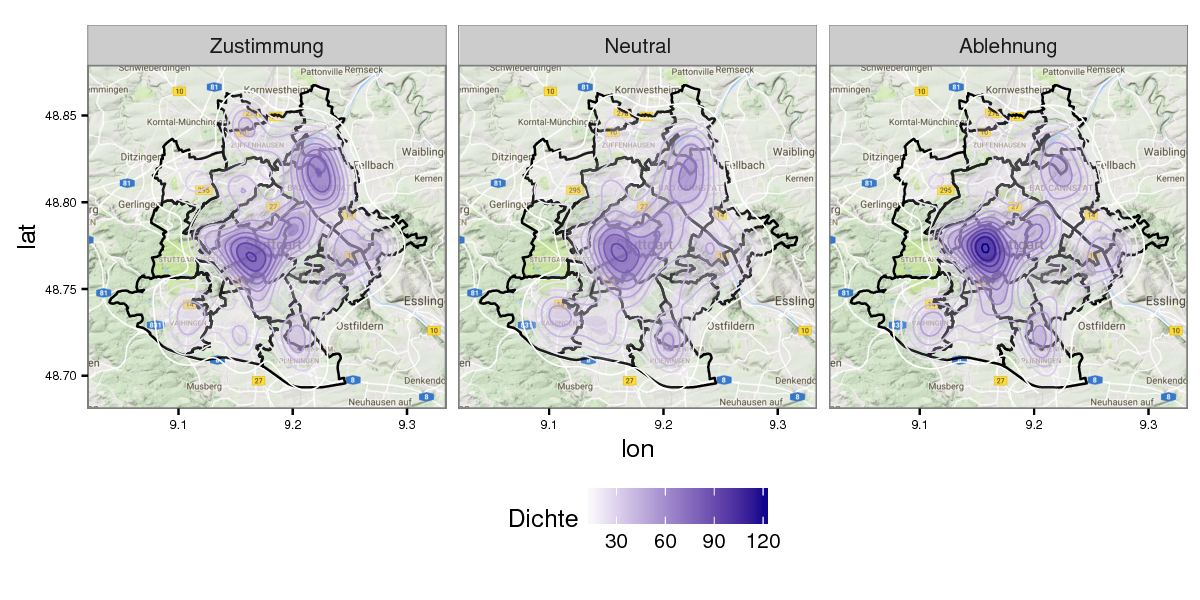
\includegraphics[scale=0.8]{Pictures/XYStuttgart3.png}
 \caption{Kontur Plot der absoluten Anzahl der Gruppenbeobachtungen zur Meinung zu Stuttgart 21 in drei Gruppen. Quelle der Hintergrundgrafik: \cite{google}}
 \label{XYStuttgart3}
 \end{center}
\end{figure}

Die \textit{Zustimmung} zeigt offensichtliche räumliche Muster. Im Zentrum und im Nordosten ist sie höher als im Rest 
der Stadt. Der räumliche Trend der \textit{Ablehnung} ist schwächer ausgeprägt. Es zeigt sich jedoch, dass der Bereich 
der Innenstadt, sowie die südlichen Stadtbereiche etwas höhere Dichten bei der \textit{Ablehnung} aufweisen. Die 
Beobachtungen der Kategorie \textit{neutral} sind eher gleichmäßig über die Stadt verteilt.\\
Abbildung \ref{XYWohnG5} zeigt die Dichte der Beobachtungen der fünf Kategorien zur Bewertung der Wohngegend. Hier zeigt sich ein deutlich ausgeprägteres räumliches Muster als bei der Meinung zu Stuttgart 21. Die Beobachtungen der Klasse \textit{sehr gut} häufen sich sehr stark im Innenstadtbereich und im Süden. Die Kategorie \textit{gut} verteilt sich relativ homogen über das gesamte Stadtgebiet mit einer etwas stärkeren Konzentration in der Innenstadt und im Nordosten. Bei der Klasse \textit{neutral} zeigt sich eine stärkere Konzentration auf den Osten und Nordosten der Stadt. Praktisch alle \textit{schlechten} und \textit{sehr schlechten} Bewertungen sind deutlich abgegrenzt im Osten und Nordosten lokalisiert. Hierbei ist zu erwähnen, dass der Anteil der Personen, die ihre Wohngegend mit \textit{schlecht} oder \textit{sehr schlecht} bewertet haben sehr gering ist Abbildung \ref{endogene}.\\

\begin{figure}[h]
 \begin{center}
 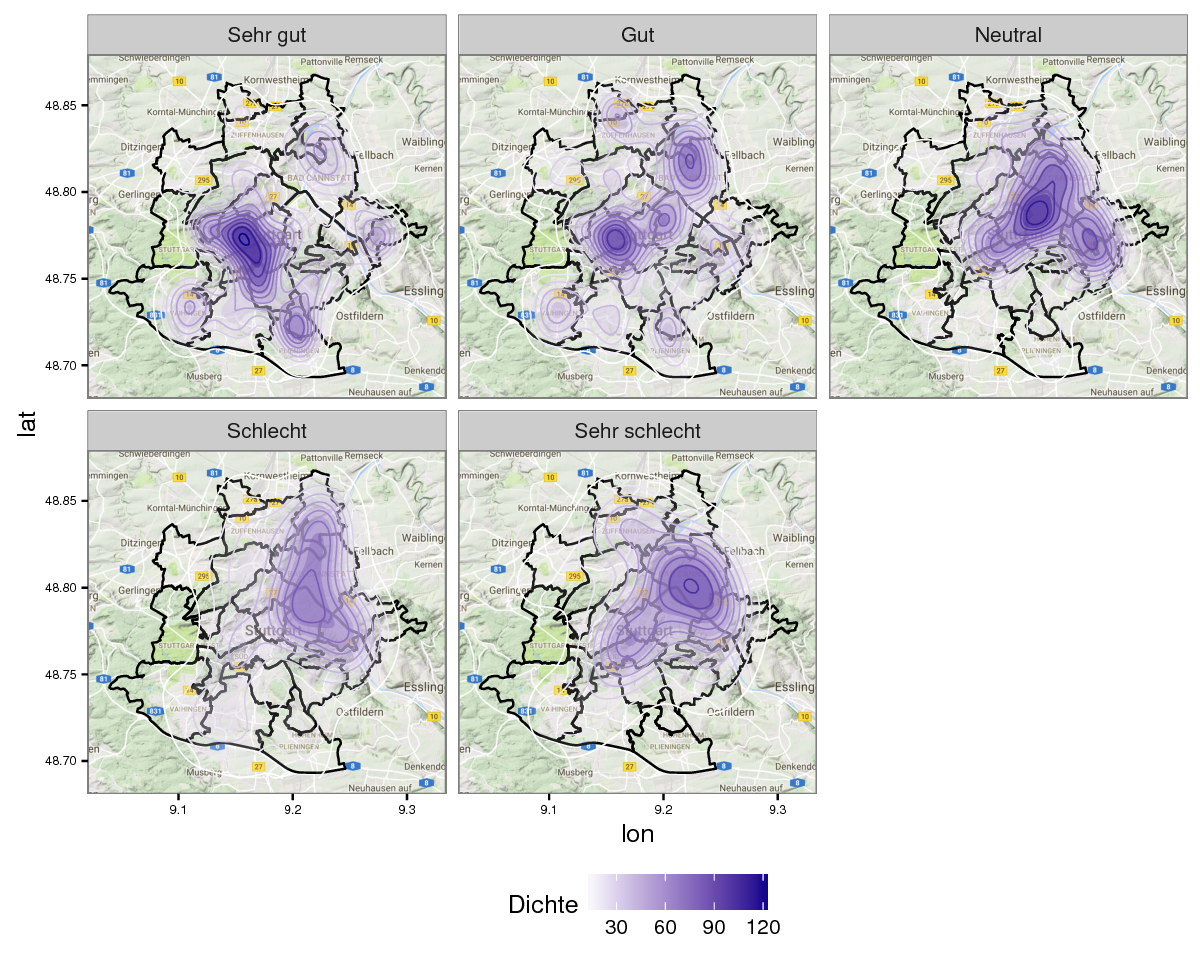
\includegraphics[scale=0.8]{Pictures/XYWohnG5.png}
 \caption{Kontur Plot der absoluten Anzahl der Gruppenbeobachtungen zur Wohnzufriedenheit in fünf Gruppen. Quelle der Hintergrundgrafik: \cite{google}}
 \label{XYWohnG5}
 \end{center}
\end{figure}


Im folgenden werden die diskreten räumlichen Informationen auf Stadtbezirksebene beschrieben. Es werden 23 Stadtbezirke 
unterschieden. Im Gegensatz zur stetigen Beobachtungsdichte werden die Beobachtungen nach Regionen aggregiert 
dargestellt. Dies hat den Vorteil, dass eine relative Anteilsdarstellung möglich wird (Abbildung 
\ref{BStuttgart21}). Die absoluten Häufigkeiten sind jedoch nicht dargestellt. Analog zur stetigen Darstellung 
(Abbildung \ref{XYStuttgart3}) ist auch hier zu sehen, dass die Bürger des Nordostens eine positivere Meinung zu 
Stuttgart 21 haben als die Bürger aus dem Süden. Die \textit{neutrale} Klasse hat in allen Bezirken einen geringeren 
Anteil und es ist kein räumliches Muster erkennbar. Die entsprechenden Anteilsgrafiken mit fünf Klassen für die 
Bewertung der Wohngegend sind im Anhang verfügbar (Abbildung \ref{BWohn}). Wie in Abbildung \ref{XYWohnG5} bereits 
angedeutet, zeigen sich negative Wohngebietseinschätzungen vor allem im Nordosten.

\begin{figure}[h]
 \begin{center}
 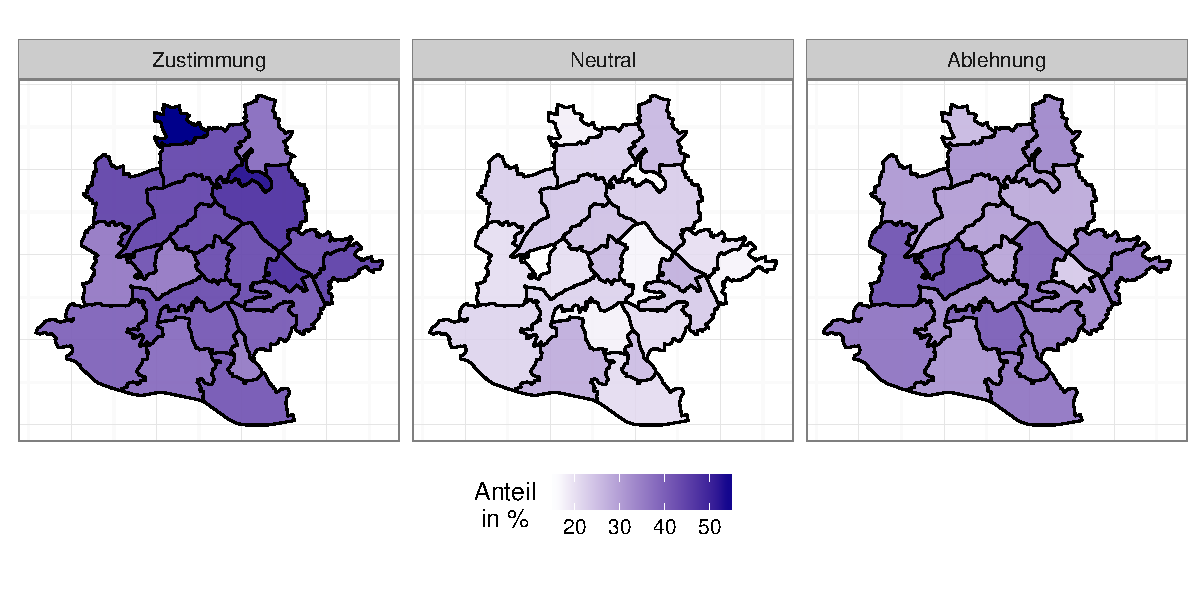
\includegraphics[scale=0.8]{Pictures/BStuttgart3}
 \caption{Anteile zur Meinung zu Stuttgart 21 nach Stadtbezirken.}
 \label{BStuttgart21}
 \end{center}
\end{figure}

Die dritte und letzte untersuchte räumliche Agrregationsebene ist die Stadtteilebene. Abbildung \ref{SStuttgart21} 
zeigt die räumliche Verteilung von \textit{Zustimmung}, \textit{Ablehnung} und \textit{neutraler} Haltung. Wie aus 
Tabelle \ref{Datensatz} hervorgeht, ist die Stadtteilebene deutlich feiner Aufgelöst als die Bezirksebene. Dies führt in 
der Abbildung dazu, dass einige Stadtteile mit geringer Gesamteinwohneranzahl in einer oder mehreren Klassen keine 
Beobachtungen zeigen. Es gibt im Umkehrschluss auch Stadtteile, in denen eine Klasse zu 100 \% vertreten ist. 
Außerdem gibt es in dieser Aggregationsebene sogar Stadtteile ohne jede Beobachtung, wie z. B. das Benzviertel im 
Innenstadtbereich oder die bereits angesprochenen Lagen im Westen.

\begin{figure}[h]
 \begin{center}
 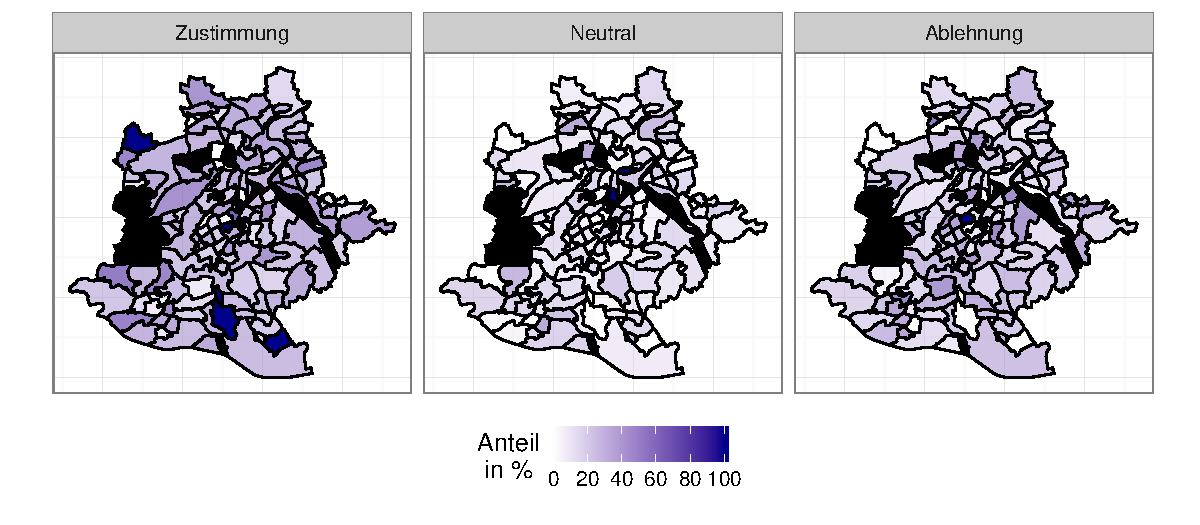
\includegraphics[scale=0.8]{Pictures/SStuttgart3}
 \caption{Anteile der Meinung zu Stuttgart 21 nach Stadtteilen.}
 \label{SStuttgart21}
 \end{center}
\end{figure}

Diese Stadtteile werden in den Diagrammen schwarz dargestellt. Wegen der feineren Auflösung ergibt sich ein 
mosaikartiges, visuell schwerer interpretierbares Bild. In keiner der drei Klassen lässt sich eine klare Struktur oder 
ein räumliches Muster erkennen. Die Anteile auf Stadtteileebene zu der Bewertung der Wohngegend sind im Anhang 
verfügbar \ref{SWohn}. Hier zeigt sich ein ähnlich schwer differenzierbares Muster wie bei der Meinung zu Stuttgart 21. 
Wegen der deutlichen Unterschiede in den Anteilen der fünf Gruppen sind die Farbskalen nicht einheitlich, sondern 
unterscheiden sich in den Diagrammen.\\

\subsubsection{Melderegister}
Die erste Datei an der die Modelle Anwendung finden sollen ist eine personenbezogene Auswertung aus dem Melderegister 
Stuttgarts vom 31.01.2011. Der Auszug umfasst alle volljährigen Einwohner Stuttgarts außer Bewohner von Anstalten und 
Pflegeheimen. Mit einem Stichprobenumfang von 470.190 Bürgern liegt der Melderegisterauszug also sehr nah an 
der Grundgesamtheit von 573.104 Bürgern, die 2011 mit Hauptwohnsitz in Stuttgart gemeldet waren \cite{bundesamt}. Insgesamt wurden 8 sozioökonomische Variablen erhoben. Bei allen Datensätzen liegt der Wohnsitz als 
kontinuierliche Gauß-Krüger Geokoordinate vor. Um eine kleinräumige Extrapolation mit diskreten räumlichen 
Informationen vornehmen zu können, wurden die Stadtteil- und Stadtbezirksinformationen an die Datensätze des 
Melderegisters angehängt. Hierzu wurden die Stadtteil- und Stadtbezirkspolygone, welche uns von der Stadt Stuttgart für 
die Analyse zur Verfügung gestellt wurden, über eine räumliche Abfrage mit den Melderegisterdatensätzen verknüpft. Die 
geographische Verknüpfung wurde mit dem freien Geoinformationssystem QGIS \textcolor{red}{(REF QGIS)} durchgeführt. Die 
Projektdatei mit der Geoabfrage (\textit{Geographische\_Abfrage.QGS}) sowie die Shapefiledateien 
(\textit{Stadtteile\_netto.SHP}) liegen dieser Arbeit digital bei. Wie in den Tabellen \ref{Datensatz} und 
\ref{Var_Buergerumfrage} ersichtlich, eignen sich nicht alle Variablen zur Extrapolation, da nicht alle Variablen in 
jeder Umfrage erhoben wurden. Es ergibt sich ein Überschneidungsbereich der fünf sozioökonomischen Variablen 
\textit{Altersklasse Befragter}, \textit{Geschlecht}, \textit{Nationalität}, \textit{Familienstand} und 
\textit{Personenzahl im Haushalt}. \textcolor{red}{IN TAB 2 BRAUCHEN WIR DIE SPALTE MODLLEIRUNG EIGENTLICH NICHT MEHR 
ODER? ICH HABE DIE VARIABLEN Z.T. UMBEBENANNT, DAMIT SIE GLEICH HEIßen WIE IN TAB 1. AUßERDEM SIND JA NACH DEM 
UMKODIEREN BEI DER ALTERSKLASSE NUR NOCH  6 AUSPR. ICH WÜRDE DAS IN DER TAB. 2 ANPASSEN WAS MEINST DU?}

\begin{table}[h]
\centering
\caption{Sozioökonomische und geographische Variablen des Melderegisters und deren Anzahl der Ausprägungen.}
\label{Var_Buergerumfrage}
\adjustbox{max height=\dimexpr\textheight-5.5cm\relax,
           max width=\textwidth}{
\begin{tabular}{l|c|c}
\multicolumn{3}{l}{Anzahl Beobachtungen: 470.190}     \\ 
\hline \hline
\textbf{Variable} & \textbf{Modellierung} & \textbf{Anzahl Ausprägungen}  \\ \hline
\multicolumn{1}{l|}{Altersklasse Befragter} &  Nicht Parametrisch & 14 \\ \hline
\multicolumn{1}{l|}{Geschlecht} &  Parametrisch  & 2 \\ \hline
\multicolumn{1}{l|}{Nationalität} & Parametrisch  & 2 \\ \hline
\multicolumn{1}{l|}{Familienstand} & Parametrisch & 4 \\ \hline
\multicolumn{1}{l|}{Personenzahl im Haushalt} &  Nicht Parametrisch  & 5 \\ \hline
\multicolumn{1}{l|}{Wohndauer} & Nicht Parametrisch  & 3 \\ \hline
\multicolumn{1}{l|}{ALG II Quote} & Nicht Parametrisch  & 9 \\ \hline
\multicolumn{1}{l|}{Ein/Zweifamilienhäuser}& Nicht Parametrisch & 8 \\ \hline 
\multicolumn{1}{l|}{Gauß-Krüger} & Tensorprodukt-Splines & \\ \hline \hline
\end{tabular}

}
\end{table}

\subsubsection{Zensus}
Im Rahmen der bundesweiten Volkszählung von 2011 wurde in Stuttgart eine Gebäude- und Wohnungszählung durchgeführt. Diese Datei umfasst 380.238 Bürger Datensätze (Tabelle \ref{Var_Zensus}). Da bei der Zählung auch für die Fragestellung dieser Arbeit relevante sozioökonomische Variablen 
erhoben wurden, eignet sich diese Umfrage ebenfalls zur kleinräumige Extrapolation. Die diskreten geographischen 
Angaben wurden analog zum Vorgehen beim Melderegister per geographischer Abfrage ergänzt. Für die kleinräumige Extrapolation kommen 
die gleichen sozioökonomischen Variablen wie beim Melderegister in Frage. 

\begin{table}[h]
\centering
\caption{Erhobene sozioökonomische und geographische Variablen der Gebäude- und Wohnungszählung im Rahmen des Zensus und deren Anzahl der Ausprägungen.}
\label{Var_Zensus}
\adjustbox{max height=\dimexpr\textheight-5.5cm\relax,
           max width=\textwidth}{
\begin{tabular}{l|c|c}
\multicolumn{3}{l}{Anzahl Beobachtungen: 380.238}     \\ 
\hline \hline
\textbf{Variable} & \textbf{Modellierung} & \textbf{Mögliche Ausprägungen}  \\ \hline
\multicolumn{1}{l|}{Altersklasse Befragter} &  Nicht Parametrisch & 9 \\ \hline
\multicolumn{1}{l|}{Geschlecht} & Parametrisch  & 2 \\ \hline
\multicolumn{1}{l|}{Nationalität} & Parametrisch  & 2 \\ \hline
\multicolumn{1}{l|}{Familienstand} & Parametrisch & 4 \\ \hline
\multicolumn{1}{l|}{Personenzahl im Haushalt} &  Nicht Parametrisch  & 6 \\ \hline
\multicolumn{1}{l|}{Wohnfläche} & Nicht Parametrisch & 24 \\ \hline
\multicolumn{1}{l|}{Stellung Beruf} & Parametrisch  & 9 \\ \hline
\multicolumn{1}{l|}{Beamter}& Parametrisch & 2 \\ \hline 
\multicolumn{1}{l|}{Gebäudetyp}& Parametrisch & 10 \\ \hline
\multicolumn{1}{l|}{Gebäudenutzung}& Parametrisch & 2 \\ \hline
\multicolumn{1}{l|}{Gauß-Krüger} & Tensorprodukt-Splines & \\ \hline \hline
\end{tabular}

}
\end{table}

\newpage

\subsection{Statistische Methoden}

Zur Vorstellung der statistischen Methoden dieser Arbeit wird zunächst das Geoadditiven Modell, welches zur Parametrisierung und anschließenden Extrapolation genutzt wird, eingeführt. Dabei wird insbesondere auf die modelspezifischen Besonderheiten der endogenen Variablen eingegangen, sowie auf die Modellierung der unterschiedlichen Kovariablen, die im vorangegangen Kapitel erläutert wurden. Außerdem wird kurz auf die Implementierung am Rechner eingegangen. Anschließend erfolgt eine Darstellung der Methoden, die zur Ermittlung des jeweils besten Modells für beide endogene Variablen genutzt werden.

\subsubsection{Schrittweiser AIC Vergleich}
Basierend auf den vorhergegangenen Analysen des Beamten- und Eigenheimanteils in Stuttgart, die uns zur Verfügung standen wurde eine Funktion zur schrittweisen AIC \cite{Akaike1981} Berechnung programmiert, die zur Identifikation der geeignetsten sozioökonomischen Kovariablenkombination dient (siehe digitaler Anhang \textit{stepAIC.R}). In der Funktion werden mithilfe der \texttt{gam()} Funktion des \texttt{mgcv} 
Paketes \cite{Wood2011} generaliserte additive Modelle mit unterschiedlichen Kovariablen erstellt und deren AIC 
berechnet. Vor dem Aufruf der Funktion müssen die abhängige Variable, die Verteilungsannahme des Regressionsmodelles, 
die Gewichtungen der Einzelbeobachtungen und unveränderliche Kovariablen definiert werden. Außerdem muss eingeschätzt 
werden, welche der veränderlichen Kovariablen parametrisch oder semiparametrisch als Spline in das Modell eingehen. Es 
wird zunächst der AIC des einfachsten, nur aus den fest vorgegebenen Kovariablen bestehenden Modells berechnet. In 
Iteration eins werden alle veränderlichen Kovariablen einzeln nacheinander in die Modellformel aufgenommen und es wird 
jeweils ein GAM erstellt sowie dessen AIC berechnet. Die Kovariablen gehen zunächst entsprechend der vorigen Eingabe parametrisch 
oder semiparametrisch ein. Außerdem werden alle vorab als nichtparametrisch eingeschätzten Variablen zusätzlich als parametrischer Trend geprüft. Falls die Hinzunahme mindestens einer Kovariable in Iteration eins zu einer Reduktion des AIC 
führt, wird diejenige Kovariable, welche zu dem Modell mit dem kleinsten AIC führt zur Modellformel hinzugefügt. Falls 
das Modell nur mit den festen Modellbestandteilen bereits den geringsten AIC zeigt ist die Modellwahl folglich in 
Iteration eins bereits beendet.\\ 
Andernfalls setzt sich das Ausgangsmodell für Iteration zwei aus den festen 
Kovariablen und einer weiteren Kovariable zusammen. In Iteration zwei werden wie zuvor alle verbleibenden Kovariablen 
zunächst nacheinander zur aktuellen Modellformel hinzugefügt. Wenn die Kovariable mit dem geringsten AIC gefunden ist 
(falls diese existiert und das Modell aus Iteration eins nicht bereits das geeignetste ist), werden alle veränderbaren 
Kovariablen in Iteration zwei nochmals nacheinander eliminiert. Das Modell mit dem geringsten AIC bildet das 
Ausgangsmodell der nächsten Iteration. Dies wird wiederholt bis in einer Iteration kein Modell mit einem geringeren AIC 
als in der vorigen Iteration parametrisiert werden kann. Um die Laufzeit der Funktion zu begrenzen, wurde auf die 
Analyse von Wechselwirkungen zwischen den Kovariablen verzichtet. Wechselwirkungen können jedoch als unveränderliche 
Modellbestandteile eingehen. In dieser Arbeit wird der Einfluss unterschiedlicher räumlicher Effekte auf die Modellqualität analysiert. Die räumlichen Effekte wurden deshalb im schrittweisen AIC Vergleich nicht berücksichtigt. Sie gingen, sofern das betrachtete Modell über einen räumlichen Effekt verfügte, als unveränderlicher Modellbestandteil ein.

\subsubsection{Verwendete Modelle}
Alle zu modellierenden endogenen Variablen besitzen kategoriale Merkmale. Ziel der Modellierung ist also  die Ausprägungswahrscheinlichkeit dieser Kategorien vorherzusagen. Da negative Wahrscheinlichkeiten sowie Wahrscheinlichkeiten über 1 nicht sinnvoll interpretierbar sind, muss demnach sichergestellt sein, dass die endogene Variable des Regressionsmodells nur stetige Werte zwischen 0 und 1 einnehmen kann. Da sich diese Vorgabe mit einfachen linearen Regressionsmodellen normalerweise nicht einhalten lässt, sind diese folglich für die Fragestellung dieser Arbeit ungeeignet. Des Weiteren weisen kategoriale Regressionsmodelle häufig keine Normalverteilung auf \cite[p. 277]{fahrmeir2013regression}, was zusätzlich gegen einfache lineare Modelle mit gewöhnlicher kleinste-Quadrate-Schätzung spricht. Im Gegensatz zu einfachen linearen Regression kann der lineare Prädiktor


\begin{equation} \label{linPraed}
\eta_{i} =\mathbf{x}'_i \boldsymbol{\beta},
\end{equation}

in generalisierten linearen Modellen (GLM) über eine Response-Funktion $h$ transformiert werden. Die Response-Variable hängt demnach nicht mehr direkt von einer linearen Kombination der Modellkovariablen, sondern von deren Transformation ab. Die Wahl der Response-Funktion hängt von der Fragestellung und von der Skalierung der Response-Variable ab. $h$ kann jede monoton ansteigende Funktion sein. Um den gewünschten Wertebereich zwischen 0 und 1 sicherzustellen wird der lineare Prädiktor bei kategorialen Regressionen häufig über eine logistische Response-Funktion transformiert. Im Falle einer binären Response-Variable ergibt sich durch die logistische Transformation nach \cite[p. 270 f.]{fahrmeir2013regression} das binäre Logit Modell

\begin{equation} \label{logit}
h(\eta)=\frac{\exp(\eta)}{1+\exp(\eta)},
\end{equation}

wobei die Response nach der Transformation einer Bernoulli Verteilung folgt. Durch Datengruppierung kann die Rechenzeit reduziert werden. Die absoluten Gruppenhäufigkeiten folgen dann einer Binomial- und die relativen Gruppenhäufigkeiten skalierten Binomialverteilungen \cite[p. 277 f.]{fahrmeir2013regression}.\\
In einem kumulativen Modell kann die Reihenfolge der Ausprägungen einer ordinalskalierten Response explizit berücksichtigt werden \cite[p.334 ff.]{fahrmeir2013regression}. Dem kumulativen Modell unterliegt die Annahme, dass in jedem Datensatz eine kontinuierliche (unbekannte) latente Variable $u_i$ existiert, deren Ausprägung die Kategoriezugehörigkeit dieser Beobachtung bestimmt. Dem Modell unterliegt des Weiteren die Annahme, dass diese latente Variable durch einen linearen Prädiktor

\begin{equation}
u_i=-\mathbf{x}'_i \boldsymbol{\tilde{\beta}}+\varepsilon,
\end{equation}

über die Modellkovariablen vorhergesagt werden kann. Ein Datensatz zeigt die Ausprägung $r$, wenn ihre latente Variable zwischen den Schwellenwerten $\theta_{r-1}$ und $\theta_r$ liegt. Um sicherzustellen, dass diese Schwellenwerte identifizierbar sind, hat der lineare Prädiktor selbst keinen Intercept. Wie zuvor im binären Fall, wird der lineare Prädiktor über eine kumulative Verteilungsfunktion transformiert. Über die Verteilung $F$ des Fehlers des linearen Prädiktors  $\varepsilon_i$ um die latente Variable $u_i$ kann die Wahrscheinlichkeit jeder Kategorie der Response-Variablen als 

\begin{equation}
P(y_i=r)=F(\theta_r+\mathbf{x}'_i \boldsymbol{\tilde{\beta}})-F(\theta_{r-1}+\mathbf{x}'_i \boldsymbol{\tilde{\beta}})
\end{equation}

berechnet werden. Da es sich um geordnete Kategorien handelt, muss zur Berechnung der Wahrscheinlichkeit der Zugehörigkeit zur Gruppe $r$ nur die Wahrscheinlichkeitsdichte zwischen den Schwellenwerten $\theta_{r}$ und $\theta_{r-1}$ berechnet werden. Wenn die in der Literatur vorgeschlagene logistische Transformation gewählt wird \cite[p. 335]{fahrmeir2013regression}, ergibt sich demnach das kumulative Logit Modell

\begin{equation}
P(y_i\leq r)=\frac{\exp(\theta_r+\mathbf{x}'_i \boldsymbol{\tilde{\beta}})}{\exp(1+\exp(\theta_r+\mathbf{x}'_i \boldsymbol{\tilde{\beta}}))}.
\end{equation}

Die exogenen Variablen, mit denen das Modell für die räumliche Extrapolation parametrisiert werden soll, sind sehr heterogen. Es kommen sowohl nominal- als auch kardinalskalierte sozioökonomischen Variablen in Frage (Abbildung \ref{endogene}, Tabelle \ref{Datensatz}). Während ein linearer Prädiktor zur Beschreibung des Zusammenhangs zwischen ordinalskalierten Kovariablen und kategorieller Response-Variablen ausreichend ist, zeigen kardinal skalierte Variablen oft einen nichtlinearen Zusammenhang \cite[p. 9]{fahrmeir2009regression}. Der in GLM vorausgesetzte lineare Prädiktor (Formel \ref{linPraed}) ist demnach für die Daten dieser Arbeit zu unflexibel. Aufgrund dieser Ausgangslage haben flexiblere Modelle voraussichtlich Vorteile gegenüber GLM.\\
In generalisierten additiven Modellen (GAM) können lineare und nichtlineare Effekte sehr flexibel in einem Modell verbunden werden, da die Terme des Prädiktors in GAM nicht auf lineare Funktionen beschränkt sind (Formel \ref{SplinePraed}). Während die Kovariablen mit linearen Effekten $\mathbf{x}_i$, analog zum GLM, durch den linearen Prädiktor modelliert werden, können die nichtlinearen Kovariableneffekte $\mathbf{z}_i$ über sehr flexible, semi- bzw. nonparametrische Splines modelliert werden \cite[p. 1 f.]{wood2016}.

\begin{equation} \label{SplinePraed}
\eta_{i} =\mathbf{x}'_i \boldsymbol{\beta}+f_{i}(\mathbf{z}_{i})
\end{equation}

GAM bieten sich also immer an, wenn lineare und nichtlineare Kovariableneffekte in einem Modell berücksichtigt werden sollen oder wenn die genauen Formen der Effekte unbekannt sind. Zur Modellierung der univariaten nichtlinearen Effekte dieser Arbeit wurden penalisierte Basissplines (P-Splines) verwendet \cite{eilers1996}. Dieser Spline-Typ ist der Gruppe der semiparametrischen Modelle zuzuordnen, da die Spline-Kurve, im Gegensatz zu z. B. Kernel-Regressionen, über zusammengesetzte Polynome konstruiert wird. Das Modell setzt sich also aus einer großen Zahl abstrakter Variablen zusammen, die keine direkte Interpretation zulassen \cite[p. 1]{eilers1996}. Basissplines (B-Splines) haben gegenüber anderen Spline-Typen, wie z. B. \textit{Truncated-Power-Series-Basis-Splines}, numerische Vorteile da die Regressionsparameter relativ kleine Werte annehmen und die abschnittsweisen Polynome untereinander weniger stark korrelliert sind \cite[p. 426]{fahrmeir2013regression}. B-Splines können über die Methode der kleinsten Quadrate gelöst werden \cite[p. 430]{fahrmeir2013regression} und benötigen daher verhältnismäßig wenig Rechenzeit. Die Qualität der Anpassung eines polynomischen Splines hängt maßgeblich von Anzahl und Lage der Übergänge (Knoten) der zusammengesetzten Polynome ab. Hier liegt ein weiterer Vorteil der B-Splines. Während die optimale Glättung bei anderen Spline-Typen zum Teil aufwendig über Modellauswahlstrategien hergeleitet werden muss, kann bei B-Splines eine relativ simple Penalisierung definiert werden \cite[p. 89 f.]{eilers1996}. Hierzu wird zunächst ein sehr flexibles Modell mit einer großen Anzahl Spline-Basen definiert, welches ex-post über den Penalisierungsterm geglättet wird. Die Krümmung von zweifach differenzierbaren Funktionen kann über das Integral der zweiten Ableitung ermittelt werden. Bei B-Splines kann dieses Integral einfach über die quadrierten zweiten Abweichungen der Spline Funktion approximiert werden \cite[p. 433]{fahrmeir2013regression}. Die penalisierte Spline Kurve (P-Spline) kann daher über die penalisierte Methode der kleinsten Quadrate geschätzt werden. In die Schätzung gehen nur die Rohdaten und der Glättungsparameter $\lambda$ ein \cite[p. 93]{eilers1996}. Über $\lambda$ kann der Trade-Off zwischen Glättung und Anpassung eingestellt werden. Das R Paket \texttt{mgcv} \cite{Wood2011} liefert zudem unterschiedliche Möglichkeiten $\lambda$ auf Grundlage der Eingangsdaten, z. B. per \textit{generalisierter Kreuzvalidierung} \cite[p. 480]{fahrmeir2013regression} oder \textit{Restricted Maximum Likelihood} \cite{wood2016}[p. 32 f.], zu optimieren. P-Splines sind demnach sehr komfortabel anzuwenden da sie außer den Eingangsdaten keine Benutzereingaben erfordern und die Rechenzeit gering ist.\\
Analog zu GLM können in GAM ebenfalls Response-Funktionen und unterschiedliche Verteilungsannahmen der Response Variablen definiert werden \cite[p. 448]{fahrmeir2013regression}. Die Ausprägungswahrscheinlichkeiten für binäre Responses können in GAM demnach über eine logistische Response-Funktion (Formel \ref{logit}) modelliert werden. Unterschiedlich ist lediglich der Prädiktor (Formel \ref{SplinePraed}). Eben dies gilt für geordnete kategoriale Modelle. Als kumulative Verteilungsfunktion für Wahrscheinlichkeitsdichte $F$ ist im \textit{mgcv} Paket ebenfalls die logistische Transformationsfunktion implementiert \cite[p. 22]{wood2016}.\\
Bei räumlich expliziten Daten kann häufig nicht von der Unabhängigkeit der Beobachtungen ausgegangen werden. Wie die visuelle Interpretation der Rohdaten nahelegt (z. B. Abbildung \ref{BStuttgart21}) zeigen räumlich nähere Beobachtungen mit höherer Wahrscheinlichkeit die gleiche Ausprägung als weiter entferntere. Es existiert offensichtlich räumliche Korrelation in den Daten. Das Modell lässt sich also voraussichtlich durch Hinzunahme eines räumlichen Effekts verbessern. Wenn in einem GAM räumliche Effekte berücksichtigt werden, spricht man von einem geoadditiven Modellen \cite[p. 540]{fahrmeir2013regression}. In dieser Arbeit wurden zwei unterschiedliche Methoden zur Berücksichtigung des räumlichen Effektes verwendet. Zunächst gingen die Gauß-Krüger Geokoordinaten $s_x$ und $s_y$ kontinuierlich in Form eines penalisierten \textit{Tensorprodukt Thin Plate Splines} (TP-Spline) ein. Diese Spline Form hat sich wegen ihrer radialen Struktur für geographische Koordinaten als vorteilhaft erwiesen \cite[p. 354]{gu1993}. Des weiteren sind TP-Splines bei großen Datenmengen für multivariate Einflüsse in Bezug auf die Rechenzeit effizient \cite[p. 95 f.]{wood2003}.

\begin{equation}
\eta_{i} =\mathbf{x}'_i \boldsymbol{\beta}+f_{i}(\mathbf{z}_{i})+f_{spat}(s_{x_i},s_{y_i})
\end{equation}

Die zweite in dieser Arbeit vorgestellte Möglichkeit der Berücksichtigung räumlicher Effekte ist das Markov-Zufallsfeld. Der räumliche Effekt kann nach \cite[p. 541]{fahrmeir2013regression} als 'Stellvertreter für unbeobachtete räumliche Variablen' interpretiert werden. Der räumliche Effekt ist also eine Proxy-Variable für unbekannte Variablen, die sich in diskreten Regionen unterscheiden. Der Prädiktor des geoadditiven Modells mit Markov-Zufallsfeld kann als

\begin{equation}
\eta_{i} =\mathbf{x}'_i \boldsymbol{\beta}+f_{i}(\mathbf{z}_{i})+f_{spat}(s_i)
\end{equation}


ausgedrückt werden \cite[p. 541]{fahrmeir2013regression}. Wobei $s_i$ die Zugehörigkeit zu einer diskreten Region kodiert. Im Regressionsmodell hat jede Region folglich einen eigenen Koeffizienten. Um geglättete räumliche Strukturen zu erhalten wird jeder Koeffizient über quadrierte Abweichung der Koeffizienten der Nachbarregionen penalisiert \cite[p. 522]{fahrmeir2013regression}. Regionen, die eine gemeinsame Grenze mit $s_i$ teilen werden als Nachbarn erster Ordnung bezeichnet. Nur diese werden für die Glättung berücksichtigt.
Ein praktisches Problem in der Implementierung eines Markov-Randomfields mit dem \texttt{mgcv} Paket ist, dass in jeder Region mindestens eine Beobachtung jeder Kategorie der abhängigen Variable vorkommen muss. Wie bereits in dem Kapitel zum Parametrisierungsdatensatz gezeigt fehlen insbesondere auf Stadtteilebene häufig einzelne Beobachtungen einer Kategorie oder auch Beobachtungen im Allgemeinen in einzelnen Regionen. \textcolor{red}{Habe neue Sätze eingefügt} Es müssen aus methodischer Sicht nicht zwingend in der Region und Kategorie Beobachtungen vorhanden sein, jedoch erlaube die \texttt{gam()} Funktion aus dem \texttt{mgcv} keine leeren Region-Kategorie Kombinationen. Um die Implementierung dennoch möglich zu machen wurde eine Funktion erstellt, die partiell oder komplett fehlende Beobachtungen durch Pseudo-Beobachtungen ersetzt und mit Null gewichtet. Alle anderen (echten) Beobachtungen werden mit eins gewichtet (siehe digitaler Anhang \textit{PseudoB.R}).

\subsubsection{Reklassifizierung}

Das verfahren der Reklassifizierung wird genutzt, um die Prognosequalität der Modelle innerhalb der Stichprobe zu überprüfen.Im Gegensatz zur nachfolgenden Kreuzvaildierung zeichnet sich die Reklassifizierung durch eine simple Implementation und geringe Rechenzeit aus, was ihr zusätzlich auch in dieser Arbeit Attraktivität verleiht. Bei dem Verfahren selbst wird der vollständige Stichprobendatensatz genutzt um mithilfe des vorher parametrisierten Modells die Klassen der Beobachtungen in dem Datensatz zu Prognostizieren. Anschließend lässt sich ermitteln wie oft Beobachtungen in die richtige oder eine falsche Klasse prognostiziert wurde. Dies ist möglich sowohl für die Modelle insgesamt, als auch für die jeweils einzelnen Klassen.


\subsubsection{Kreuzvalidierung}
Die Kreuzvalidierung gibt im Gegensatz zur bereits beschriebenen Reklassifizierung , die Möglichkeit die Modelle auf ihre Prognosequalität außerhalb der Stichprobe zu prüfen und ist deshalb von besonderem Interesse.
Für die Modellerstellung der additiven Modelle lag eine Stichprobe von 3.143 Beobachtungen vor. Informationen zur Grundgesamtheit dieser Stichprobe lagen nicht vor. Die Qualität der parametrisierten Modelle ließ sich folglich nicht anhand einer Grundgesamtheit validieren, sondern musste an der Stichprobe selbst eingeschätzt werden. Die erstellten Modelle wurden an anderen Daten als den Parametrisierungsdaten angewendet. Aus diesem Grunde ist war vor allem die Modellqualität außerhalb der Parametrisierungsdaten interessant. Daher wurde eine \textit{Leave-One-Out} Kreuzvalidierung durchgeführt \cite[p. 149]{fahrmeir2013regression}, in welcher jeweils eine Beobachtung zufällig entfernt wurde. Mit den verbliebenen Datensätzen wurde das additive Modell, welches sich zuvor im schrittweisen AIC Vergleich als am vorteilhaftesten herausgestellt hat, neu parametrisiert und die entfernte Beobachtung mit diesem Modell vorhergesagt. Dies wurde so lange wiederholt bis jeder Datensatz einmal entfernt (und geschätzt) wurde. Mit diesen Daten ließ sich eine Statistik zur Reklassifikation der Beobachtungen außerhalb der Stichprobe erstellen.


\subsubsection{Prognoseintervalle}
Die Intervalle zu den Punktschätzungen liefern zusätzliche wichtige Informationen, da die Punkt"-schätzungen alleine keine Angaben zur Unsicherheit beinhalten. Das Prognoseintervall gibt an, mit welcher Wahrscheinlichkeit die unbekannte wahre Punktschätzung von einer Konfidenzregion überdeckt wird. Mit dem Vertrauensintervall erhält man die Relation der Unsicherheit zur Punktschätzung und somit ein weiteres Modellgütemerkmal \cite[p. 471]{fahrmeir2013regression}. Des weiteren wurden die Intervalle genutzt um Überdeckungswahrscheinlichkeiten des Volksabstimmungsergebnisses \cite{Amt} zu berechnen. Grundsätzlich gibt es die Möglichkeiten die Intervalle entweder aus Modelleigenschaften abzuleiten oder Bootstrap-Intervalle durch wiederholte zufällige Modellreparametrisierungen und Punktschätzungen zu berechnen. Bei ersterem Vorgehen unterliegen die Intervallberechnungen, je nach gewählter Berechnungsmethode, asymptotischen Eigenschaften oder Verteilungsannahmen. So wird zur analytischen Berechnung von Score-Konfidenzintervallen \cite[p. 64 ff.]{held2008}, welche den Vorteil haben, dass sie invariant gegenüber eindeutigen Parametertransformationen sind, beispielsweise die Fischer-Information benötigt. Sie sind deshalb oft nur schwer analytisch zu berechnen \cite[p. 74]{held2008}. Andere Intervalle, wie beispielsweise das Wald-Konfidenzintervall, sind obligatorisch symmetrisch \cite[p. 60]{held2008} und werden der wahren Datenverteilung daher oft nicht gerecht. Bei beiden Intervallen hängt die tatsächliche Überdeckungswahrscheinlichkeit der unbekannten wahren Parameter bei binärer Response Variable zudem von der Parameterausprägung sowie der Beobachtungsanzahl der Modellstichprobe ab und entspricht deshalb in ungünstigen Kombinationen nicht der nominellen, also der gewünschten Überdeckungswahrscheinlichkeit \cite{Int}. 
\\Bootstrap Intervalle hingegen können für jede Form der statistischen Inferenz berechnet werden \cite{diciccio1996}. Da in dieser Arbeit Modelle mit unterschiedlichen Verteilungsannahmen und unterschiedlichen räumlichen Effekten verglichen werden, bietet es sich an auf die verteilungsunabhängigen Bootstrap-Intervallschätzungen zurückzugreifen. Von Interesse sind weniger die Intervalle um die Modellparameter als vielmehr die Intervalle um die Punktschätzungen, also die einzelnen Hochrechnungen. Dementsprechend wurden Bootstrap-Intervalle für jede einzelne Punktschätzung berechnet. Zur Berechnung der Intervalle wurde jedes Modell 1.000 mal mit einer Zufallsstichprobe (\textit{Ziehen-mit-Zurücklegen}) aus der Parameterisierungsstichprobe reprametrisiert. Um den Einfluss des Stichprobenumfangs zu eliminieren, enthielt jede Stichprobe die tatsächliche Anzahl der Beobachtungen. Mit jedem neuparametrisierten Modell wurde eine kleinräumige Extrapolation durchgeführt. Die Hochrechnungsergebnisse wurden genutzt um die arithmetischen Mittel, die Mediane sowie untere und obere 95 \% Perzentile der Punktschätzungen zu berechnen.

\subsubsection{Validierung}
Ziel der Validierung ist es, die prognostizierten Anteile aus dem gewählten Modell mit den wahren Anteilen aus der 
Volksabstimmung \cite{Amt} zu vergleichen, um eine Aussage über die Qualität der geschätzten Prognosemodelle geben zu 
können. Die Validierung erfolgt auf Stadtteil- und Bezirksebene, sowie für das Gesamtergebnis der Stadt Stuttgart. Dazu 
werden insbesondere zwei statistische Gütemaße verwendet, das erste soll den Punktschätzer valideren und das zweite wird benutzt, um den Intervallschätzer zu validieren.\\
Bei der Wahl des Schätzers geht es zum einen darum, einen möglichst erwartungstreuen als auch effizienten Schätzer, d.h. mit minimaler Varianz zu finden. Als geeignetes Gütemaß hat sich die mittlere quadratische Abweichung (MSE) erwiesen, da sie sowohl die Varianz, als 
auch die quadrierte Verzerrung berücksichtigt. Für einen Schätzer $\hat{\theta}$ von dem wahren Parameter $\theta$ ist die MSE definiert als
$$
\text{MSE } = \mathbb{E}[(\hat{\theta} - \theta)^2],
$$
wobei sich durch den mittleren Verschiebungssatz der Varianz zeigen lässt, dass
$$
\text{MSE } = \mathbb{V}(\hat{\theta}) + \mathbb{B}(\hat{\theta})^2
$$
gilt.Die MSE lässt also auch zu einem gewissen Maße verzerrte Schätzer zu, was in bestimmten Situationen sehr hilfreich sein kann. Zudem hat ein konsistenter Schätzer die Eigenschaft, dass die mittlere 
quadratische Abweichung bei unendlich groß werdender Stichprobe gen Null konvergiert \cite[p. 201]{HOG}. Ein weiteres 
Kriterium ist die Überdeckungswahrscheinlichkeit. Sie gibt an, mit welcher Wahrscheinlichkeit das geschätzte 
Konfidenzintervall den wahren Wert enthält und ist nach \cite{zhang} in der großen Stichprobe definiert als

$$
\lim\limits_{n \rightarrow \infty}{P(\theta \in S_{1-\alpha}(\hat{\theta})) < 1-\alpha},
$$

wobei $S_{1-\alpha}$ die Konfidenzregion von $\theta$ angibt. Erwartet wird hier also, dass die Überdeckungs"-wahrscheinlichkeit knapp unter dem
Konfidenzniveau liegt. Mögliche größere Abweichungen können durch die Approximation einer diskreten Verteilung 
durch eine stetige Verteilung resultieren, was z.B. oft bei der Approximation der Binomial- durch die Normalverteilung 
vorkommt \cite[p. 102]{Int}.

\section{Ergebnisse}
Nachdem im Material und Methoden Teil zunächst die Datensätze und statistischen Methoden vorgestellt wurden, zeigt dieses Kapitel die daraus entstanden Ergebnisse. Dafür werden zunächst die geschätzten Parameter der verschiedenen Modelle und die geschätzten Modelle in Gänze analysiert. Insgesamt wurden zur Meinung zu Stuttgart 21 sechs geoadditive Modelle geschätzt, drei Modelle mit drei Ausprägungen der abhängigen Variable und drei Modelle mit zwei Ausprägungen. Beide Modellierungsmöglichkeiten wurden dabei einmal mit jedem der drei räumlichen Effekte parametrisiert. Zudem wurde in allen Fällen noch jeweils ein Modell nur mit räumlichem Effekt und ein Modell ohne räumlichem Effekt geschätzt. Für die Bewertung der Wohngegend wurde nur ein Fall mit fünf Klassen geschätzt, aber jeweils auch mit drei räumlichen Effekten und Modellen mit- und ohne räumlichem Effekt. Insgesamt ergibt das 18 geschätzte Modelle für die Meinung zu Stuttgart 21 und 9 Modelle für die Bewertung der Wohngegend. Um diese hohe Anzahl zu reduzieren werden anhand der Modellwahlkriterien aus dem vorangegangen Kapitel nach und nach Modelle eliminiert, die auf Grund dieser Kriterien als bestes Modell zur Extrapolation ausscheiden. Zum Schluss werden mit den zuletzt verbliebenen Modellen die Extrapolationen auf die Grundgesamtheit vorgenommen, um dann die beiden finalen Modelle zu finden. 


\subsection{Schrittweiser AIC Vergleich}
Durch die Kovariablenwahl mit Hilfe der schrittweisen AIC Funktion ist sichergestellt, dass die Kombination der sozioökonomischen Variablen einen sinnvollen Kompromiss aus Modellanpassung und Modellkomplexibilität widerspiegelt. Die Wechselwirkung zwischen \textit{Personenzahl im Haushalt} und \textit{Altersklasse des Befragten}, welche den AIC im Fall des drei Klassenmodells zur Meinung von Stuttgart 21 minderte, wurden zusammen mit dem räumlichem Effekt fest vorgegeben. Zur exemplarischen Darstellung der Funktion wurde Abbildung \ref{AIC} erstellt. Sie zeigt die Konvergenz des AIC für das Aktuell beste Modell, für welches wiederum die verbleibenden Kovariablen nacheinander getestet werden. Zu sehen ist, dass die Funktion für die Bewertung der Wohngegend bereits nach vier äußeren Iterationen keine Verbesserung des AIC mehr erreichen kann und die optimale Modellkomplexität gefunden wurde. Für die Modelle zur Meinung zu Stuttgart 21 ist die optimale Modellkomplexität nach fünf bzw. sechs äußeren Iterationen gefunden.

\begin{figure}[h]
 \begin{center}
 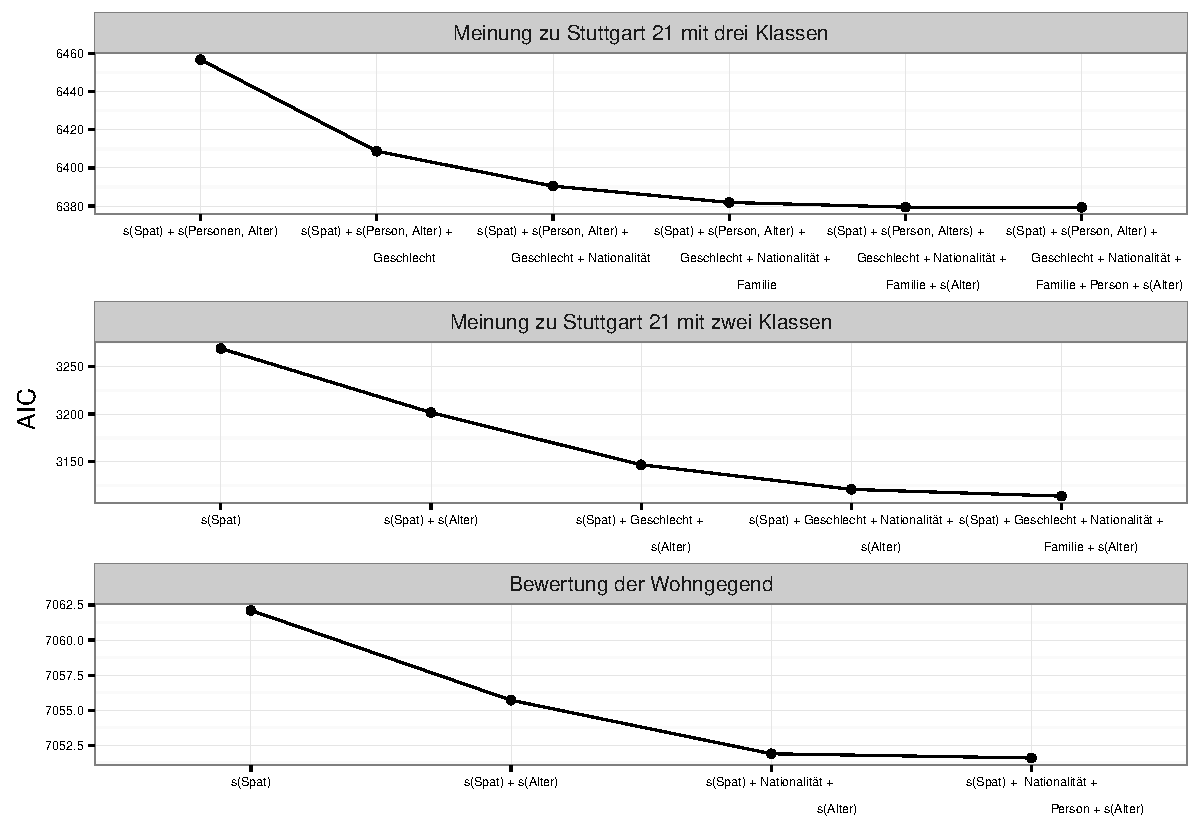
\includegraphics[scale=0.8]{Pictures/stepAIC}
 \caption{Konvergenz der äußeren Schleife der \textit{stepAIC} Funktion zur Ermittlung der optimalen Parameterkombinationen exemplarisch für alle Response Möglichkeiten mit Gauß-Krüger Informationen}
 \label{AIC}
 \end{center}
\end{figure}

Damit weist das drei Klassenmodell zur Meinung zu Stuttgart 21 die höchste Modellkomplexität auf. Ein interessantes Ergebnis der \textit{stepAIC} Funktion ist zudem, dass neben einer Hinzunahme der Wechselwirkung auch die Hinzunahme der Anzahl der im Haushalt lebenden Personen für das zwei Klassenmodell keine Verbesserung des AIC erreicht, obwohl beide Modelle im Prinzip das gleiche Problem behandeln. Die geringste Komplexität weißt das Modell zur Bewertung der Wohngegend auf. Es ist deutlich erkennbar, dass die Hinzunahme weiterer Kovariablen nach dem räumlichem Effekt nur eine sehr geringe Verbesserung des AIC bewirken, so ist die Differenz zwischen dem Modell nur mit räumlichem Effekt und dem bestem Modell nur ca 10 Punkte. Im Gegensatz dazu konnte durch die Hinzunahme vom Kovariablen im zwei Klassenmodell zur Meinung zu Stauttgart 21 von ca 150 Punkten erreicht werden. Zu beachten ist jedoch auch, dass dies exemplarisch für die Gauss-Krüger Informationen ist, für die anderen räumlichen Effekte sind auch deutlich andere Parameterkombinationen anhand des AIC entstanden.
Insgesamt deutet das AIC für den drei Klassen Fall auf das Geoadditive Modell mit den Gauß-Krüger Informationen als qualitativ höchstes Modell hin. Beim zwei Klassen Fall schneidet das Geoadditive Modell in jedem Fall am besten ab, wobei hier das Modell mit Stadtteilen als räumlichem Effekt die höchste Qualität laut dem AIC aufweist.


\subsection{Modelle}
Über die schrittweise AIC Analyse wurde die geeignetste Kombination der sozioökonomischen Variablen jedes Modells festgelegt. In Tabelle \ref{stepAIC} wird der zusätzliche Effekt der räumlichen Komponente auf die Modelle betrachtet. Um die Einflüsse der räumlichen Effekte isoliert bewerten zu können, blieb die zuvor ermittelte Kovariablenkombination innerhalb eines Modells gleich. Die Kombination der sozioökonomischen Kovariablen ist in Tabelle \ref{stepAIC} folglich in jeder Zeile gleich. Jedes geoadditive Modell wird mit einem Modell ohne räumlichen Effekt sowie einem Modell nur mit dem räumlichen Effekt verglichen. Beim Vergleich muss beachtet werden, dass die AIC der Modelle auf Stadtteilebene nicht direkt mit den kontinuierlichen Modellen und den Modellen auf Stadtbezirksebene vergleichbar sind. Durch die Pseudobeobachtungen sind die Stichprobenumfänge nicht gleich.\\

\begin{table}[h]
\centering
\caption{AIC der erstellten Modelle.}
\label{stepAIC}
\begin{tabular}{llccc}
\hline \hline
\multicolumn{5}{c}{Meinung zu Stuttgart 21}                                                                                                                                            \\ \hline
                          & \multicolumn{1}{l|}{}             & \multicolumn{1}{c|}{\multirow{2}{*}{Geoadditives Modell}} & \multicolumn{1}{c|}{Modell ohne}       & Modell nur mit    \\
                          & \multicolumn{1}{l|}{}             & \multicolumn{1}{c|}{}                                     & \multicolumn{1}{c|}{räumlichem Effekt} & räumlichem Effekt \\ \hline
\multirow{3}{*}{Drei Kl.} & \multicolumn{1}{l|}{Gauß-Krüger} & \multicolumn{1}{c|}{6379,345}                             & \multicolumn{1}{c|}{6378,220}          & 6525,747          \\
                          & \multicolumn{1}{l|}{Bezirke}      & \multicolumn{1}{c|}{6378,267}                             & \multicolumn{1}{c|}{6379,725}              & 6528,284          \\
                          & \multicolumn{1}{l|}{Stadtteile}   & \multicolumn{1}{c|}{6456,706}                               & \multicolumn{1}{c|}{6535,627}          & 6605,946          \\ \hline
\multirow{3}{*}{Zwei Kl.} & \multicolumn{1}{l|}{Gauß-Krüger} & \multicolumn{1}{c|}{3114,141}                             & \multicolumn{1}{c|}{3116,130}           & 3268,484          \\
                          & \multicolumn{1}{l|}{Bezirke}      & \multicolumn{1}{c|}{3115,858}                             & \multicolumn{1}{c|}{3116,130}           & 3271,325          \\
                          & \multicolumn{1}{l|}{Stadtteile}   & \multicolumn{1}{c|}{3149,607}                              & \multicolumn{1}{c|}{3180,433}          & 3298,017          \\ \hline
\multicolumn{5}{c}{Bewertung der Wohngegend}                                                                                                                                           \\ \hline
                          & \multicolumn{1}{l|}{}             & \multicolumn{1}{c|}{\multirow{2}{*}{Geoadditives Modell}} & \multicolumn{1}{c|}{Modell ohne}       & Modell nur mit    \\
                          & \multicolumn{1}{l|}{}             & \multicolumn{1}{c|}{}                                     & \multicolumn{1}{c|}{räumlichem Effekt} & räumlichem Effekt \\ \hline
                          & \multicolumn{1}{l|}{Gauß-Krüger} & \multicolumn{1}{c|}{7054,163}                             & \multicolumn{1}{c|}{7318,815}          & 7064,751          \\
                          & \multicolumn{1}{l|}{Bezirke}      & \multicolumn{1}{c|}{7175,601}                             & \multicolumn{1}{c|}{7318,815}          & 7197,003          \\
                          & \multicolumn{1}{l|}{Stadtteile}   & \multicolumn{1}{c|}{8252,374}                             & \multicolumn{1}{c|}{8567,358}          & 8750,801          \\ \hline \hline
\end{tabular}
\end{table}
Bei der Meinung zu Stuttgart 21 in drei sowie in zwei Kategorien lässt sich erkennen, dass die geoadditiven Modelle stets gleiche oder etwas bessere AIC zeigen als die Modelle ohne räumlichen Effekt. Die Modelle ohne sozioökonomische Kovariablen schneiden stets am schlechtesten ab. Im direkten Vergleich haben die sozioökonomischen Variablen also einen höheren Erklärungsgehalt als die räumlichen Effekte. Die Form des räumlichen Effektes spielt eine untergeordnete Rolle. Es spielt im Hinblick auf die relative Modellqualität kaum eine Rolle, ob der räumliche Effekt kontinuierlich oder diskret auf Bezirksebene modelliert modelliert wird.\\
Bei der Bewertung der Wohngegend wirkt sich der räumliche Effekt sehr viel stärker auf die relative Modellqualität aus. Alle Modelle mit räumlichen Effekten zeigen stets die niedrigsten AIC. Der Vergleich der Modelle nur mit sozioökonomischen Variablen zu den Modellen ohne sozioökonomische Variablen offenbart, dass die räumlichen Effekt sogar wichtiger als die sozioökonomischen Kovariablen sind. Der Vergleich der räumlichen Effekte zeigt, dass das kontinuierliche geoadditive Modell gegenüber den diskreten Modellen vorteilhaft ist.\\
Zusammenfassend ist zu sagen, dass die geoadditiven Modelle tendenziell zumindest gleichwertig zu den GAM ohne räumlichen Effekt sind. Im folgenden Verlauf der Arbeit werden deshalb nur noch geoadditive verwendet.\\
Das erste geoadditive Modell zur Modellierung der Meinung zu Stuttgart 21 mit dreikategorialer Response (\textit{Zustimmung}, \textit{Neutral} und \textit{Ablehnung}) und kontinuierlichem räumlichen Trend wird im Folgenden näher erläutert. Aus Abbildung \ref{GKParam} und \textcolor{red}{Tabelle X} geht die Signifikanz der Modellparameter hervor. Hierbei ist zu beachten, dass \textit{Zustimmung} mit 1 und \textit{Ablehnung} mit 3 kodiert wurde. Je höher der Effekt, desto höher ist also die Wahrscheinlichkeit der \textit{Ablehnung}. Die \textit{Altersklasse des Befragten} zeigte einen stark nichtlinearen Trend. Die Wahrscheinlichkeit der Ablehnungswahrscheinlichkeit ist in den jüngeren Altersklassen bis 2 am geringsten. Sie steigt bis zu ihrem Höhepunkt bei Altersklasse  4,5 an und fällt dann relativ stark wieder ab. \textcolor{red}{gucken, was die AKL bedeutetn} Die Personenzahl im Haushalt ging, entgegen der Erwartungen, parametrisch in das Modell ein. Der Effekt zeigt einen stark negativen linearen Trend. Die Wahrscheinlichkeit der \textit{Ablehnung} ist also in Single-Haushalten mit deutlichem Abstand am höchsten. Die Kategorien des Familienstands unterscheiden sich zwar nicht signifikant von 0, werden jedoch aufgrund der leichten AIC Verringerung dennoch berücksichtigt. Es ist ersichtlich, dass \textit{geschiedene} und \textit{ledige} Bürger eher eine ablehnende Haltung gegenüber Stuttgart 21 zeigen \textit{verheiratete} oder \textit{verwitwete}. Deutlicher sind die Effekte der Nationalität und des Geschlechts. \textit{Deutsche} Bürger zeigen eine signifikant höhere Ablehnungswahrscheinlichkeit als ausländische Bürger. Der Unterschied zwischen den Geschlechtern ist etwa ebenso stark. Männer haben eine geringere Ablehnungswahrscheinlichkeit als Frauen. Die Kovariablenausprägungen finden sich in näherungsweise gleicher Ausprägung in allen dreikategorialen geoadditiven Vorhersagemodellen der Meinung zu Stuttgart 21 (TAB) \textcolor{red}{Tabellen der GAM im Anhang}. Ausnahme bildet einzig der Familienstand im diskreten räumlichen Modell auf Stadtbezirksebene, welcher nach schrittweiser AIC Analyse nicht in dieses Modell eingeflossen ist.\\
Die visuelle Überprüfung der unterschiedlichen Parameterausprägungen der räumlichen Effekte (Abbildung \ref{rEffS21}) offenbart ein deutliches Nord-Süd Gefälle der Ablehnungswahrscheinlichkeit. In \textit{Stammheim} im äußersten Norden ist der räumliche Einfluss auf den Prädiktor bei allen drei räumlichen Modellen unter -0,1 und damit am geringsten in ganz Stuttgart. Des weiteren ist die Ablehnungswahrscheinlichkeit in den nördlichen Bezirken \textit{Zuffenhausen}, \textit{Münster} und \textit{Bad Cannstadt} im Vergleich zu allen Stadtteilen sehr gering. Die Ablehnungswahrscheinlichkeit steigt tendenziell in südlicher Richtung. Etwa in der Mitte der Stadt, verlaufend vom Stadtbezirk \textit{Weilimsdorf} im Westen über \textit{Feuerbach}, \textit{Mitte} und \textit{Wangen} bis nach \textit{Obertürkheim} im Osten, ist der räumliche Modelleinfluss nahe 0. Südlich dieser Linie steigen die Parameterausprägungen tendenziell in südwestlicher Richtung. Im Bezirk \textit{Vaihingen} sind mit deutlichem Abstand die höchste Ablehnungswahrscheinlichkeiten zu sehen. Dieser grundsätzliche Trend ist in allen drei Modellen ähnlich ausgeprägt. Nach Stadtteilen aufgelöst (Abbildung \ref{rEffS21} (c)) lassen sich die räumlichen Trends jedoch noch kleinräumiger darstellen. Innerhalb des südlichen Bereichs (in dem die Ablehnung tendenziell höher ist) sind in dieser Auflösungsebene Hot-Spots sichtbar. So zeigt sich, dass die Ablehnungswahrscheinlichkeit innerhalb \textit{Vaihingens} inhomogen verteilt ist. Das Stadtteil \textit{Vaihingen-Mitte} zeigt die höchste Parameterausprägung aller Stuttgarter Stadtteile. Die Parameter der anderen Stadtteile \textit{Vaihingens} sind deutlich kleiner. Aus diesen Grunde ist die Skala der Parameterausprägung auf Stadtteilebene (Abbildung \ref{rEffS21} (c)) höher als auf Stadtbezirksebene Abbildung \ref{rEffS21} (b)). Weitere nennenswerte Abweichungen der Stadtteile innerhalb ihrer Bezirke ergeben sich nur noch in dem relativ großen Bezirk \textit{West}. Während die Haltung in \textit{Solitude} eher \textit{zustimmend} ist, nehmen Bürger aus \textit{Kräherwald} und \textit{Wildpark} eher eine Ablehnende Haltung ein. Dieser Stadtbezirk nimmt eine Sonderstellung ein, da er sehr wenige, in den Stadtteilen \textit{Kräherwald} und \textit{Wildpark} gar keine, Beobachtungen zeigt. Die Parameterausprägung ist demnach stark von den Nachbarregionen getrieben. In allen anderen Stadtbezirken Stuttgarts ist die Parameterausprägung innerhalb der Stadtteile vergleichsweise homogen. Hier entsprechen die Parameterausprägungen der Stadtteile folglich näherungsweise den Parameterausprägungen der dazugehörigen Stadtbezirke.
\\
Die Effekte des zweikategorialen Vorhersagemodells sind, wenngleich die Kovariablenkombinationen teilweise etwas unterschiedliche sind, praktisch gleich \textcolor{red}{ANHANG}. Auch hier ist ein Nord-Süd Gefälle ersichtlich. Der Bezirk \textit{Vaihingen}, insbesondere in \textit{Vaihingen-Mitte} zeigt die höchste Ablehnungswahrscheinlichkeit, während diese in \textit{Stammheim} am geringsten ist.\\


\begin{figure}[h]
 \begin{center}
 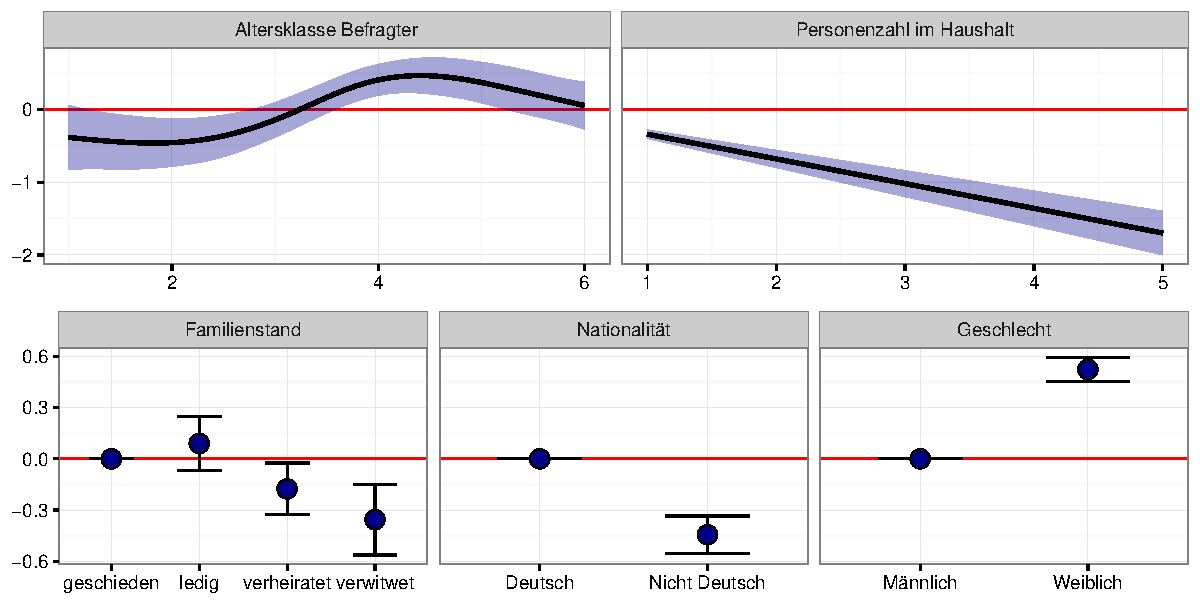
\includegraphics[scale=0.8]{Pictures/S21ModelEffects2}
 \caption{Parametrische und nonparametrische Effekte des dreikategorialen Modell zur Vorhersage der Meinung zu Stuttgart 21 mit kontinuierlichem räumlichen Trend.}
 \label{GKParam}
 \end{center}
\end{figure}


\begin{figure}[htbp]
  \centering
 %\subfigure[Kontinuierlich]{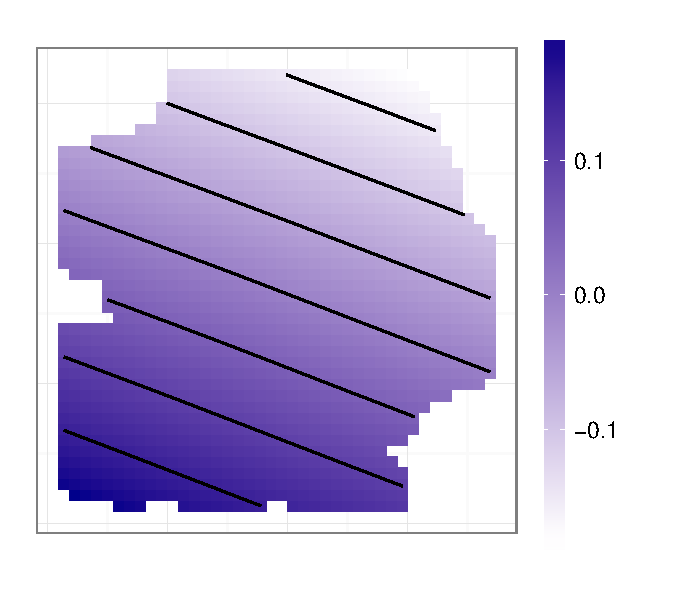
\includegraphics[scale=0.13]{Pictures/S21_3_Kont_SpatEff.png}}\quad
  \subfigure[Diskret: Stadtbezirke]{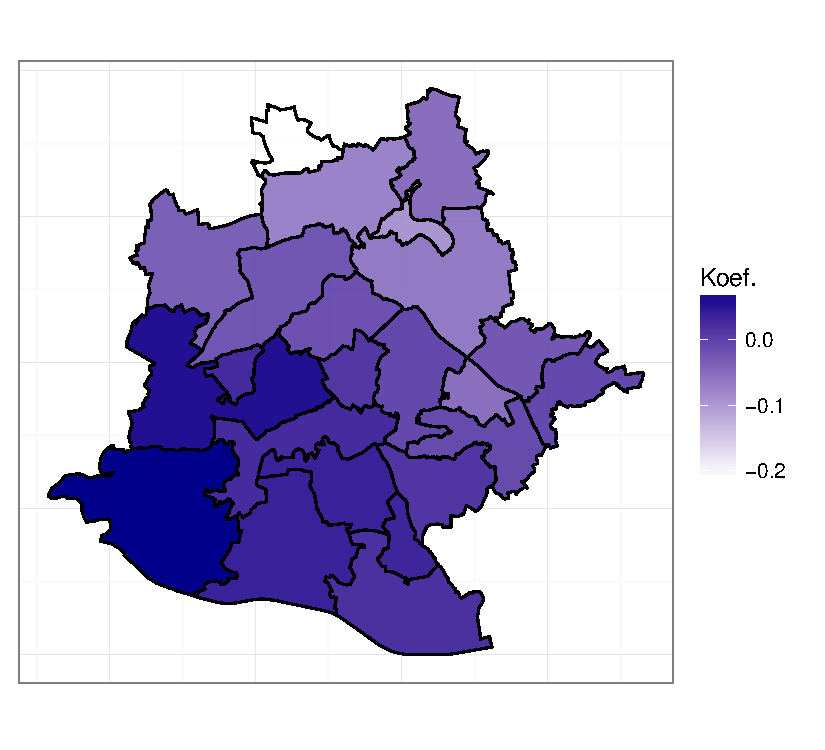
\includegraphics[scale=0.55]{Pictures/S21_3_Bezirke_SpatEff}}\quad
  \subfigure[Diskret: Stadtteile]{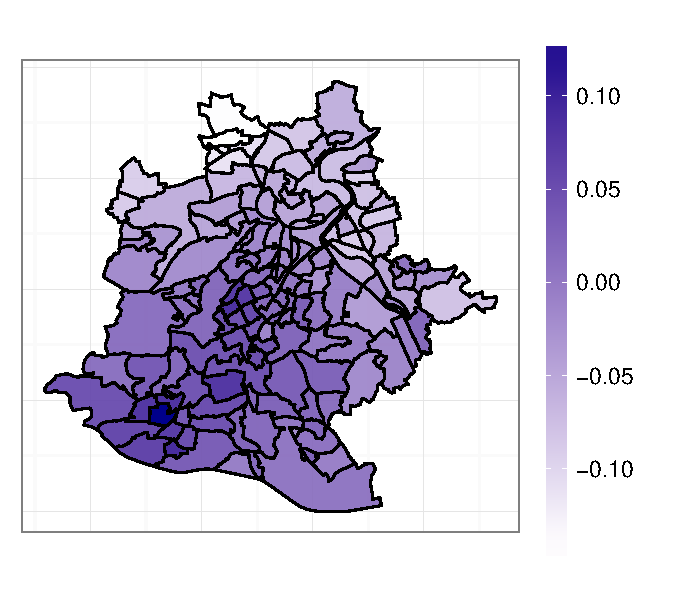
\includegraphics[scale=0.55]{Pictures/S21_3_Stadtt_SpatEff}}
  \caption{Räumliche Effekte des dreikategorialen Modell zur Vorhersage der Meinung zu Stuttgart 21.}
  \label{rEffS21}
\end{figure}



\begin{figure}[h]
 \begin{center}
 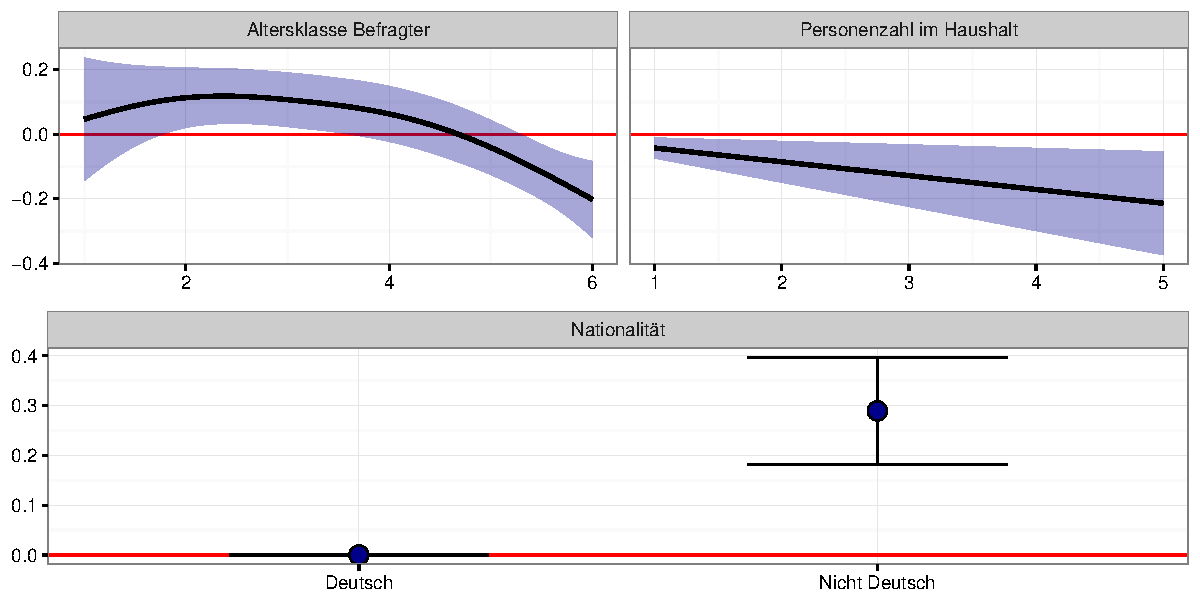
\includegraphics[scale=0.8]{Pictures/BWModelEffects2}
 \caption{Parametrische und nonparametrische Effekte des zweikategorialen Modell zur Vorhersage der Meinung zu Stuttgart 21 mit kontinuierlichem räumlichen Trend.}
 \label{BWParam}
 \end{center}
\end{figure}

\subsection{Reklassifizierung}

Die Ergebnisse der Reklassifizierung zur Meinung zu Stuttgart 21 (Tabelle \ref{evalS21}) zeigen, dass die Erfolgsquote im drei Klassenmodell zwischen 44\% und 50\% liegt und im zwei Klassenmodell zwischen 55\% und 62\% liegt. Zum Vergleich mit einem reinen Zufallsmodell, dass im drei Klassenmodell eine Erfolgswahrscheinlichkeit von 1/3 und im zwei Klassenmodell von 1/2 hat, weißen die geschätzten Modelle eine höhere Erfolgsquote auf. Auch bei einem Vergleich mit Tabelle \ref{endogene} zeigt sich, dass die geschätzten Modelle besser abschneiden, als ein triviales Wählen der immer gleichen Klasse mit der höchsten Anzahl der Beobachtungen.

\begin{table}[h]
\centering
\caption{Reklassifizierung der Meinung zu Stuttgart 21}
\label{evalS21}
\begin{tabular}{ll|c|c|c}
\hline \hline
                          &              & \multirow{2}{*}{Geoadditives Modell} & Modell ohne       & Modell nur mit    \\
                          &              &                                      & räumlichem Effekt & räumlichem Effekt \\ \hline
\multirow{3}{*}{Drei Kl.} & Gauß-Krüger & 0,4918                               & 0,4716            & 0,4732            \\
                          & Bezirke      & 0,4726                               & 0,4719            & 0,4726            \\
                          & Stadtteile   & 0,451                                & 0,4685            & 0,4449            \\ \hline
\multirow{3}{*}{Zwei Kl.} & Gauß-Krüger & 0,6193                               & 0,6104            & 0,5524            \\
                          & Bezirke      & 0,6079                               & 0,6104            & 0,5515            \\
                          & Stadtteile   & 0,6282                               & 0,6052            & 0,6099            \\ \hline \hline
\end{tabular}
\end{table}

Des weiteren ist zu sehen, dass das Geoadditive Modell in fast allen Fällen die höchste Erfolgsquote aufweist. Abweichungen bestehen im drei Klassenmodell mit Stadtteilen als räumlichem Effekt und im zwei Klassenmodell mit Bezirken als räumlichem Effekt. Außerdem ist zu beachten, dass im drei Klassenmodell das Modell nur mit räumlichem Effekt besser abschneidet als das Modell ohne räumlichem Effekt, während sich für zwei Klassen diese Situation umgekehrt hat.\\
Für die Reklassifikation der Bewertung der Wohngegend (Tabelle \ref{evalB}) ergibt sich eine Erfolgsquote zwischen 40\% und 50\%. Damit ist auch hier eine deutliche Verbesserung gegenüber rein zufälligem Wählen oder dauerhaftem Wählen einer Klasse gegeben. 

\begin{table}[h]
\centering
\caption{Reklassifizierung der Bewertung der Wohngegend}
\label{evalB}
\begin{tabular}{l|c|c|c}
\hline \hline
             & \multirow{2}{*}{Geoadditives Modell} & Modell ohne       & Modell nur mit    \\
             &                                      & räumlichem Effekt & räumlichem Effekt \\ \hline
Gauß-Krüger & 0,4922                               & 0,4461            & 0,4896            \\
Bezirke      & 0,4701                               & 0,4461            & 0,4621            \\
Stadtteile   & 0,4046                               & 0,4204            & 0,4347            \\ \hline \hline
\end{tabular}
\end{table}

Für die Modelle mit den kontinuierlichen Gauß-Krüger Informationen und den Bezirken als räumlichem Effekt hat das Geoadditive Modell die höchste Erfolgsrate, wohingegen für die Stadtteilinformationen das Modell nur mit räumlichem Effekt die beste Reklassifizierung aufweist. Insgesamt schneidet das Geoadditive Modell für beide endogene Variablen und alle drei möglichen Klassenanzahlen am besten ab. Außer bei dem zwei Klassenmodell zur Meinung zu Stuttgart 21 weisen beim Geoadditivem Modell die Gauß-Krüger Informationen als räumliche Effekte die höchste und die Stadtteile als räumliche Effekte die niedrigste Erfolgsrate auf. Da die Modelle ohne- oder nur mit räumlichem Effekt in der AIC-Untersuchung und Reklassifizierung in den meisten Fällen schlechter Abschnitten, wurden die Ansätze ohne- oder nur mit räumlichem Effekte nicht weiter verfolgt und als beste Modelle zur Extrapolation ausgeschlossen.

\subsection{Kreuzvalidierung}

Die Kreuzvalidierung wurde vorgenommen, um die Vorhersagequalität außerhalb der eigenen Stichprobe der Modelle einzuschätzen. Die Ergebnisse zur Meinung zu Stuttgart 21 (Tabelle \ref{KreuzM}) zeigen eine ähnliche Erfolgsquote wie die innerhalb der Stichprobe vorgenommene Reklassifizierung (Tabelle \ref{evalS21}). Für das drei Klassenmodell liegt der Anteil der erfolgreich Klassifizierten Beobachtungen bei ca. 49\% und im zwei Klassenmodell zwischen 60\% und 63\%. Im drei Klassen Fall kann das Modell mit Stadtteilen als räumlichem Effekt ca. 3,5\%  mehr Beobachtungen richtig zuweisen als in der Reklassifizierung und das Modell mit Bezirken als räumlichem Effekt ca. 2\% mehr, womit es insgesamt auch die höchste Erfolgsrate aufweist. Die Erfolgsquote mit den Gauß-Krüger Informationen ist in etwa gleich geblieben, ähnlich wie die Modelle im zwei Klassen Fall.
 
\begin{table}[h]
\centering
\caption{Kreuzvalidierung der Meinung zu Stuttgart 21 nach einzelnen Klassen}
\label{KreuzM}
\begin{tabular}{lcccccccccc}
\hline \hline
\multicolumn{11}{c}{Drei Klassen}                                                                                                                                                                                                        \\ \hline 
\multicolumn{1}{c}{}                                                     & \multicolumn{1}{c|}{}  & \multicolumn{3}{c|}{Gauß-Krüger}            & \multicolumn{3}{c|}{Bezirke}                 & \multicolumn{3}{c}{Stadtteile}         \\ \cline{3-11} 
                                                                         & \multicolumn{1}{c|}{}  & \multicolumn{9}{c}{Geschätzte Klasse}                                                                                                \\
                                                                         & \multicolumn{1}{c|}{}  & 1       & 2   & \multicolumn{1}{c|}{3}       & 1       & 2   & \multicolumn{1}{c|}{3}       & 1           & 2           & 3          \\ \hline
\multirow{3}{*}{\begin{tabular}[c]{@{}l@{}}Wahre \\ Klasse \end{tabular}} & \multicolumn{1}{c|}{1} & 0,756   & 0   & \multicolumn{1}{c|}{0,244}   & 0,754   & 0   & \multicolumn{1}{c|}{0,246}   & 0,746           & 0           & 0,254        \\
                                                                         & \multicolumn{1}{c|}{2} & 0,673   & 0   & \multicolumn{1}{c|}{0,327}   & 0,670   & 0   & \multicolumn{1}{c|}{0,330}   & 0,663          & 0           & 0,337        \\
                                                                         & \multicolumn{1}{c|}{3} & 0,521   & 0   & \multicolumn{1}{c|}{0,479}   & 0,511   & 0   & \multicolumn{1}{c|}{0,489}   & 0,509      & 0           & 0.491     \\ \hline
\multicolumn{2}{l|}{Klassifikation Modell}                                                        & \multicolumn{3}{c|}{\multirow{2}{*}{0,4905}} & \multicolumn{3}{c|}{\multirow{2}{*}{0,4928}} & \multicolumn{3}{c}{\multirow{2}{*}{0,4893}} \\
\multicolumn{2}{l|}{Insgeasmt}                                                                    & \multicolumn{3}{c|}{}                        & \multicolumn{3}{c|}{}                        & \multicolumn{3}{c}{}                   \\ \hline
\multicolumn{11}{c}{Zwei Klassen}                                                                                                                                                                                                        \\ \hline
                                                                         & \multicolumn{1}{l|}{}  & \multicolumn{3}{c|}{Gauß-Krüger}             & \multicolumn{3}{c|}{Bezirke}                  & \multicolumn{3}{c}{Stadtteile}         \\ \cline{3-11} 
                                                                         & \multicolumn{1}{l|}{}  & \multicolumn{9}{c}{Geschätzte Klasse}                                                                                                \\
                                                                         & \multicolumn{1}{l|}{}  & 1       & \multicolumn{2}{c|}{2}             & 1       & \multicolumn{2}{c|}{2}             & 1           & \multicolumn{2}{c}{2}    \\ \hline
Wahre                                                                    & \multicolumn{1}{l|}{1} & 0,747   & \multicolumn{2}{c|}{0,253}         & 0,732   & \multicolumn{2}{c|}{0,268}         & 0,748         & \multicolumn{2}{c}{0,252}    \\
Klasse                                                                   & \multicolumn{1}{l|}{2} & 0,538   & \multicolumn{2}{c|}{0,462}         & 0,545   & \multicolumn{2}{c|}{0,455}         & 0,516       & \multicolumn{2}{c}{0,484}    \\ \hline
\multicolumn{2}{l|}{Klassifikation Modell}                                                        & \multicolumn{3}{c|}{\multirow{2}{*}{0,6193}} & \multicolumn{3}{c|}{\multirow{2}{*}{0,6079}} & \multicolumn{3}{c}{\multirow{2}{*}{0,6286}} \\
\multicolumn{2}{l|}{Insgesamt}                                                                    & \multicolumn{3}{c|}{}                        & \multicolumn{3}{c|}{}                        & \multicolumn{3}{c}{}                   \\ \hline \hline
\end{tabular}
\end{table}

Zudem lässt sich anhand von Tabelle \ref{evalS21} die Trefferquote der einzelnen Klassen entnehmen. Die Tabelle zeigt die Anteile der Zuordnung von Beobachtungen der jeweiligen Klasse auf die eigene und jede der anderen Klassen. Die Hauptdiagonale liefert die Anteile der korrekt zugeordneten Beobachtungen. Die Einträge auf den Nebendiagonalen geben damit an, wie viele Beobachtungen einer Klasse relativ zur Gesamtzahl der Beobachtungen in eine falsche Klasse zugeordnet wurden. Markant ist, dass der zweiten Klasse in keinem Modell Beobachtungen zugeordnet wurden, weder falsch noch richtig. Mehrheitlich wurden diese der ersten Kategorie zugewiesen. Zudem ist die erste Klasse am öftesten richtig prognostiziert worden, allerdings wurden ihr auch die meisten falsch klassifizierten Beobachtungen zugeordnet. Dies gilt für alle drei Modelle. Im zwei Klassen Fall wurde das Problem der nicht geschätzten zweiten Klasse durch ihr auslassen umgangen. Allerdings findet sich auch hier ein deutlich häufigeres falsches zuordnen der zweiten Klasse in die erste als anders herum. 

\begin{table}[h]
\centering
\caption{Kreuzvalidierung der Bewertung der Wohngegend nach einzelnen Klassen}
\label{KreuzBew}
\begin{tabular}{lc|ccccccccccccccc}
\hline \hline
\multicolumn{1}{c}{}                                                     &   & \multicolumn{5}{c|}{Gauß-Krüger}              & \multicolumn{5}{c|}{Bezirke}                   & \multicolumn{5}{c}{Stadtteile}              \\ \cline{3-17} 
                                                                         &   & \multicolumn{15}{c}{Geschätzte Klasse}                                                                                                        \\
                                                                         &   & 1     & 2     & 3 & 4 & \multicolumn{1}{c|}{5} & 1     & 2     & 3 & 4 & \multicolumn{1}{c|}{5} & 1       & 2       & 3       & 4   & 5       \\ \hline
\multirow{5}{*}{\begin{tabular}[c]{@{}l@{}}W. \\ Kl.\end{tabular}} & 1 & 0,445 & 0,555 & 0 & 0 & \multicolumn{1}{c|}{0} & 0,387 & 0,613 & 0 & 0 & \multicolumn{1}{c|}{0} & 0,495   & 0,478   & 0,019   & 0   & 0,008   \\
                                                                         & 2 & 0,254 & 0,746 & 0 & 0 & \multicolumn{1}{c|}{0} & 0,252 & 0,748 & 0 & 0 & \multicolumn{1}{c|}{0} & 0,300   & 0,671   & 0,023   & 0   & 0,006   \\
                                                                         & 3 & 0,149 & 0,845 & 0 & 0 & \multicolumn{1}{c|}{0} & 0,153 & 0,847 & 0 & 0 & \multicolumn{1}{c|}{0} & 0,142   & 0,771   & 0,079   & 0   & 0,008   \\
                                                                         & 4 & 0,141 & 0,859 & 0 & 0 & \multicolumn{1}{c|}{0} & 0,141 & 0,859 & 0 & 0 & \multicolumn{1}{c|}{0} & 0,099   & 0,474   & 0,349   & 0   & 0,078   \\
                                                                         & 5 & 0,114 & 0,886 & 0 & 0 & \multicolumn{1}{c|}{0} & 0,086 & 0,914 & 0 & 0 & \multicolumn{1}{c|}{0} & 0,031   & 0,275   & 0,556   & 0   & 0,138   \\ \hline
\multicolumn{2}{l|}{Klass.}                                              & \multicolumn{5}{c|}{\multirow{3}{*}{0.4918}}   & \multicolumn{5}{c|}{\multirow{3}{*}{0,4704}}   & \multicolumn{5}{c}{\multirow{3}{*}{0,4594}} \\
\multicolumn{2}{l|}{M.}                                                  & \multicolumn{5}{c|}{}                          & \multicolumn{5}{c|}{}                          & \multicolumn{5}{c}{}                        \\
\multicolumn{2}{l|}{Insg.}                                               & \multicolumn{5}{c|}{}                          & \multicolumn{5}{c|}{}                          & \multicolumn{5}{c}{}                        \\ \hline  \hline
\end{tabular}
\end{table}

Tabelle \ref{evalB} ist analog zu Tabelle \ref{evalS21} aufgebaut. Das Ergebnis der Kreuzvalidierung für die Bewertung der Wohngegend ist, dass die Erfolgsquote zwischen ca. 46\% und 49\% liegt. Die Modelle mit Gauß-Krüger Informationen und Bezirken als räumlichen Effekten haben vergleichbar wie in der Reklassifizierung abgeschnitten. Das Modell mit den Stadtteilen hingegen weißt eine ca 5\% höhere Genauigkeit auf. Insgesamt jedoch behält das Modell mit den Gauß-Krüger Informationen die höchste Erfolgsrate. Auffällig ist auch hier, dass eine Klasse in keinem Modell Beobachtungen zugewiesen bekommen hat und zwei weitere Klassen in zwei von drei Modellen keine Beobachtungen zugewiesen bekommen haben. Abbildung \ref{endogene} gibt dabei einen Hinweis auf die Ursache dieses Phänomens, denn die Kategorien \textit{sehr gut} und \textit{gut} sind überproportional häufig im Datensatz vertreten im Vergleich zu den Klassen \textit{schlecht} und \textit{sehr schlecht}, weshalb schon durch die relative Häufigkeit die Wahrscheinlichkeit dass eine Beobachtungen in einer der letzten drei Kategorien ist, sehr klein wird. Bei der Bewertung der Wohngegend wurde am häufigsten die zweite Klasse sowohl richtig als auch falsch geschätzt.\\
Durch das relativ hohe Überschätzen einer Klasse bei beiden endogenen Variablen, sowie das totale Unterschätzen einiger Klassen, wird in der weiteren Validierung und Extrapolation auf das Vorhersagen einzelner Beobachtungen verzichtet. Stattdessen wird in einem bestimmten Gebiet über die Wahrscheinlichkeiten der Beobachtungen aggregiert und ein Anteil geschätzt, um auch geringere Wahrscheinlichkeiten für Beobachtungen zu berücksichtigen.

\subsection{Validierung}

Die Ergebnisse der Validierung sind aus Tabelle \ref{vali} ersichtlich. Die Tabelle zeigt die mittlere Quadratische Abweichung und Überdeckungswahrscheinlichkeit der prognostizierten Anteile aus den Modellen, bezogen auf die wahren Anteile aus der Volksabstimmung. Da in dieser Volksabstimmung nur Informationen zu zwei Klassen verfügbar sind, wird erwartet, dass das zwei Klassenmodell die beiden Kategorien signifikant besser prognostiziert.
Tabelle \ref{vali} ist so aufgebaut, dass die linke Spalte angibt um welche Kombination aus Modell, räumlichem Effekt und Datei zur Extrapolation es sich handelt. Die mittlere Spalte zeigt die mittlere quadratische Abweichung für die beiden Kategorien der Volksabstimmung und die rechte Spalte zeigt die Überdeckungswahrscheinlichkeit ebenfalls für diese Kategorien. Damit gibt die erste Reihe z.B. die statistischen Gütemaße für das drei Klassenmodell mit Gauß-Krüger Informationen als räumlichem Effekt aggregiert auf Bezirksebene mit dem Melderegister an. Die Prognoseintervalle zur Berechnung der Überdeckungswahrscheinlichkeit wurden mit Hilfe des Bootstraps ermittelt, sowie Mediane zur Ermittlung der Abweichung auch.

\begin{table}[h]
\centering
\caption{Vergleich der mittleren quadratischen Abweichung (MSE) und der Überdeckungs"-wahrscheinlichkeit bei allen Prognosen aus den geschätzten Modellen und den beiden Extrapolationsdateien für die Meinung zu Stuttgart 21}
\label{vali}
\begin{tabular}{llll|cc|cc}
\hline \hline
                        &                               &                          &   & \multicolumn{2}{c|}{MSE} & \multicolumn{2}{c}{Überdeckungswk.} \\
                        &                               &                          &   & Zustimmung  & Ablehnung  & Zustimmung        & Ablehnung       \\ \hline
\multirow{12}{*}{3 Kl.} & \multirow{4}{*}{Gauß-Krüger} & \multirow{2}{*}{Bez.}    & U & 0,04        & 0,749      & 1                 & 0,043           \\
                        &                               &                          & Z & 0,116       & 0,557      & 0,391             & 0               \\ \cline{3-8} 
                        &                               & \multirow{2}{*}{Sadtt.}  & U & 0,461       & 5,708      & 0,954             & 0,139           \\
                        &                               &                          & Z & 0,813       & 4,415      & 0,553             & 0,02            \\ \cline{2-8} 
                        & \multirow{4}{*}{Bezirke}      & \multirow{2}{*}{Bez.}    & U & 0,041       & 0,756      & 1                 & 0,043           \\
                        &                               &                          & Z & 0,117       & 0,562      & 0,522             & 0               \\ \cline{3-8} 
                        &                               & \multirow{2}{*}{Stadtt.} & U & 0,482       & 5,678      & 0,934             & 0,139           \\
                        &                               &                          & Z & 0,835       & 4,38       & 0,567             & 0,027           \\ \cline{2-8} 
                        & \multirow{4}{*}{Stadtteile}   & \multirow{2}{*}{Bez.}    & U & 0,032      & 0,862     &      1             &   0,043          \\
                        &                               &                          & Z & 0,148       & 0,552      &     0,478         &     0 \\ \cline{3-8} 
                        &                               & \multirow{2}{*}{Stadtt.} & U & 0,646       & 6,367       &   0,947           &   0,225  \\
                        &                               &                          & Z & 1,078        & 4,336       &   0,66           &                0,1 \\ \hline
\multirow{12}{*}{2 Kl.}  & \multirow{4}{*}{Gauß-Krüger} & \multirow{2}{*}{Bez.}   & U & 0,312      & 0,312      &     0,826           &  0,826
 \\
                        &                               &                          & Z & 0,152      & 0,152      &   0,522           &  0,522     \\ \cline{3-8} 
                        &                               & \multirow{2}{*}{Stadtt.} & U & 2,694       & 2,679     &   0,649          &  0,649   \\
                        &                               &                          & Z & 1,581       & 1,569      &  0,46            &   0,46   \\ \cline{2-8} 
                        & \multirow{4}{*}{Bezirke}      & \multirow{2}{*}{Bez.}    & U & 0,312       & 0,312      &  0,826            &   0,826    \\
                        &                               &                          & Z & 0,153       & 0,153      &  0,565            &  0,565    \\ \cline{3-8} 
                        &                               & \multirow{2}{*}{Stadtt.} & U & 2,642       & 2,645      &  0,636           &   0,636    \\
                        &                               &                          & Z & 1,527       & 1,513    &  0,433            &    0,44   
\\ \cline{2-8} 
                        & \multirow{4}{*}{Stadtteile}   & \multirow{2}{*}{Bez.}    & U & 0,524       & 0,524      &   0,043          &    0,043 \\
                        &                               &                          & Z & 0,172       & 0,172      &     0,652        &     0,652 \\ \cline{3-8} 
                        &                               & \multirow{2}{*}{Stadtt.} & U & 2,813        &  2,797      &  0,848     &  0,848 \\
                        &                               &                          & Z & 1,758        & 1,746     &    0,693     &     0,713
                         \\ \hline \hline
\end{tabular}
\end{table}

Zuerst erfolgt ein Vergleich zwischen den beiden Modellierungsmöglichkeiten. Für die Kategorie \textit{Ablehnung} zeigt die Tabelle die erwarteten Ergebnisse, sowohl die mittlere quadratische Abweichung als auch die Überdeckungswahrscheinlichkeit ist durchweg für alle Kombinationen besser im zwei Klassenmodell als im drei Klassenmodell. Die Überdeckung im drei Klassen Fall ist so gering, dass der wahre Wert nahezu nie enthalten ist. Für die Kategorie \textit{Zustimmung} ergibt sich ein komplett konträres Ergebnis. Hier ist die mittlere quadratische Abweichung bei jeder Kombination im zwei Klassenmodell deutlich geringer als im drei Klassenmodell. Auch die Überdeckungswahrscheinlichkeit ist insbesondere bei den Ergebnissen zum Melderegister signifikant höher. Zur besseren Einordnung dieser Ergebnisse wurde Abbildung \ref{vali4} erstellt. Dort ist zu sehen, dass die prognostizierten Anteile des drei Klassenmodells sehr nahe bei den wahren Anteilen liegen, wobei Punkte auf der 45 Grad Linie Beobachtungen signalisieren bei denen der wahre und der prognostizierte Anteil nahezu gleich sind. Zudem bedeutet ein Überschneiden von Prognoseintervall und 45 Grad Linie, dass das Prognoseintervall den wahren Wert überdeckt. Beim zwei Klassenmodell ist zu erkennen, dass die wahren Anteile deutlich überschätzt werden, sowohl auf Bezirks- als auch auf Stadtteilebene. Außerdem ist zu sehen, dass die Prognoseintervalle im zwei Klassenmodell eine starke Asymmetrie aufweisen, während die Prognoseintervalle des drei Klassenmodells symmetrisch sind.

\begin{figure}[h]
 \begin{center}
 
\includegraphics[scale=0.8]{Pictures/PaT2}
 \caption{Illustration geschätzte gegen wahre Anteile für Gauß-Krüger Informationen extrapoliert auf  Melderegister mit zwei und drei Klassenmodell mit 95\% Quantielen}
 \label{vali4}
 \end{center}
\end{figure}

Innerhalb des drei Klassenmodells lässt sich anhand von Tabelle \ref{vali} nicht eindeutig bestimmen, welcher räumliche Effekt das beste Modell liefert, da die größten Unterschiede sowohl bei dem MSE und der Überdeckung zwischen den Dateien auftreten, was auch darauf hinweisen kann, dass der Melderegister näher mit der Volksabstimmung übereinstimmt. Beim Melderegister liefert das Modell mit Stadtteilen als räumlichem Effekt das beste Modell auf Bezirksebene und auf Stadtteilebene das Modell mit Gauß-Krüger Informationen, wobei die Unterscheide eher marginal sind. Insgesamt kann das zwei Klassenmodell als bestes Prognosemodell verworfen werden, da das drei Klassenmodell die \textit{Zustimmung} und folglich auch die \textit{Ablehnung} deutlich genauer bestimmen kann.

\subsection{Extrapolation}

Dieses Kapitel stellt nun die Prognostizierten Anteile der Klassen für gesamt Stuttgart von den noch verbliebenen Modellen vor. Dazu zeigt Abbildung \ref{S21Alle} die Extrapolierten Anteile der Modelle zur Meinung zu Stuttgart 21. Dargestellt ist der Median als Punktschätzer zusammen mit den Prognoseintervallen. Die gestrichelten Linien stellen die respektiven Anteile in der Stichprobe dar und die durchgezogenen Linien die Anteile aus der Volksabstimmung. Bei den noch verbliebenen Modellen handelt es sich um den drei Klassen Fall mit den drei räumlichen Effekten extrapoliert auf beide Dateien und den beiden Aggregaten Bezirke und Stadtteile. Deutlich erkennbar ist ein Unterschied zwischen den Extrapolierten Anteilen aus dem Zensus und dem Melderegister. Da die Validierung ergeben hat, dass die extrapolierten Anteile aus dem Melderegister näher mit den Anteilen aus der Volksabstimmung übereinstimmen wird sich im weiteren die Analyse au die Anteile aus dem Melderegister beziehen. Vorab zu sehen ist außerdem, dass die Anteile der Stichprobe und die Anteile der wahren Ergebnisse aus der Volksabstimmung deutliche Differenzen aufweisen. Während die Stichprobe für die Klasse \textit{Zustimmung} einen Anteil von ca. 47\% zeigt, haben sich in der Volksabstimmung 52,9\% für Stuttgart 21 ausgesprochen. Natürlich aber muss dabei auch beachtet werden, dass es sich dabei um unterschiedliche Erhebungen handelt und es bei der Volksabstimmung keine neutrale Klasse erfasst wurde.\\
Auffällig sind die breiten Prognoseintervalle, die auf eine relativ hohe Unsicherheit hindeuten. Dies kann ein Indiz darauf sein, dass die Anzahl der Beobachtungen in der Stichprobe zu gering ist im Vergleich zur Grundgesamtheit. Zwischen den Modellen mit unterschiedlichen räumlichen Effekten weist das Modell mit Stadtteilen die höchste Unsicherheit auf. Die Punktschätzer von dem Modell mit Gauß-Krüger Informationen und Bezirken sind nahezu identisch. Die Punktschätzer des Stadtteilmodells weichen als einzige sichtbar ab und befinden sich am nächsten an dem Anteil der Volksabstimmung der Kategorie \textit{Zustimmung}, was allerdings nicht überbewertet werden sollte, da der Melderegister und die Volksabstimmung zu unterschiedlichen Zeitpunkten stattgefunden haben. 

\begin{figure}[h]
 \begin{center}
 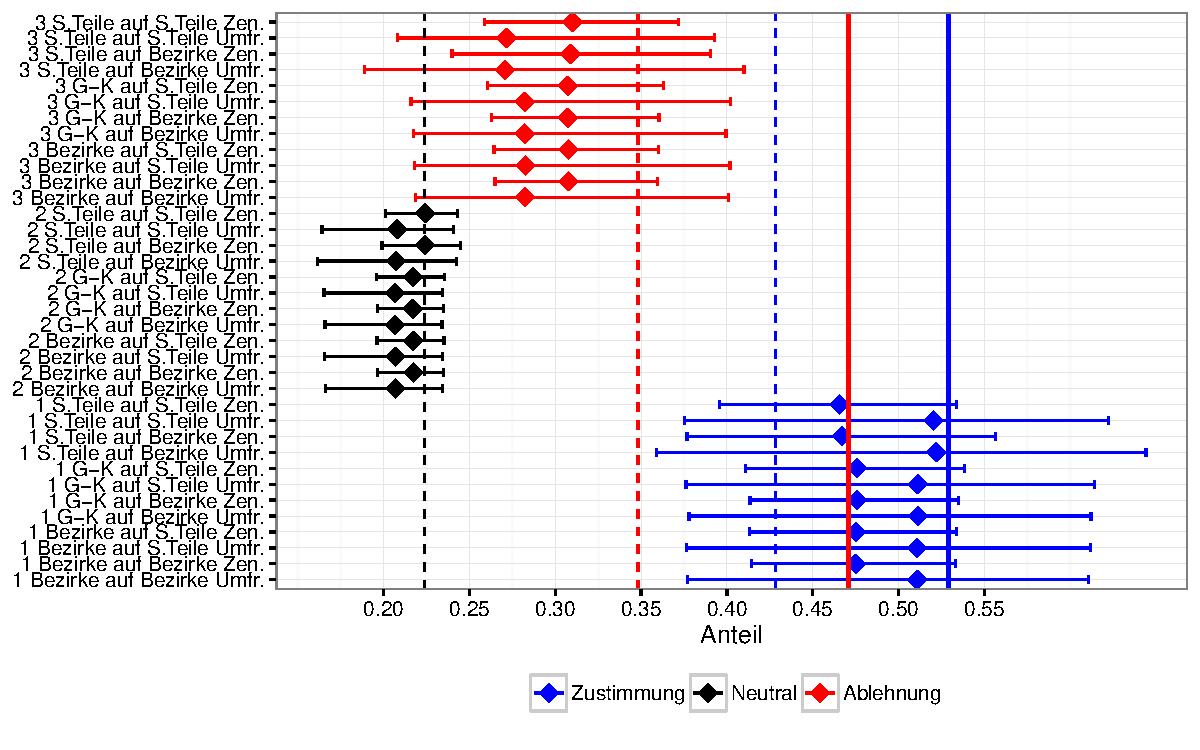
\includegraphics[scale=0.8]{Pictures/S21AlleModelle}
 \caption{Vergleich der extrapolierten Gesamtanteile für Stuttgart mit allen geschätzten Modellen und beiden Extrapolationsdateien mit den wahren Anteilen, sowie den Anteilen der Stichprobe mit 95\% Quantielen zur Meinung zu Stuttgart 21}
 \label{S21Alle}
 \end{center}
\end{figure}

Aggregiert auf Bezirksebene Für die Klasse \textit{Zustimmung} hat das Modell mit Gauß-Krüger Informationen einen Anteil von 51,12\% prognostiziert. Das Bezirksmodell hat einen Anteil von 51,09\% ergeben und das Stadtteilmodell einen Anteil von 52,06\%. Damit ergibt 1 - \textit{Zustimmung} für jedes Modell eine sehr nahe Prognose der Ablehnung aus der Volksabstimmung von 47,1\%. Gegeben den Daten und den Modellen bedeutet dies, dass Personen, die angeben eine neutrale Meinung zu haben, höchst wahrscheinlich gegen Stuttgart 21 stimmen würden. Im drei Klassen Szenario sind die prognostizierten Anteile für die \textit{neutrale} Klasse 20,65\% vom Gauß-Krüger Modell, 20,67 vom Bezirkmodell und 20,78\%. Für die Klasse \textit{Ablehnung} sind die prognostizierten Anteile in gleicher Reihenfolge 28,22\%, 28,23\% und 27,15\%. Für eine theoretische Grundgesamtheit mit drei Kategorien lässt sich nur schwierig sagen, welches Modell die beste Prognose abgibt, da auch die geschätzten Anteile für alle Klasse relativ ähnlich sind. Den bisherigen Analyse zugrunde liegend und um die Frage nach dem besten Modell zur Extrapolation zu beantworten, wird in dieser Arbeit das Modell mit den Gauß-Krüger Informationen empfohlen. Es hat die besten Ergebnisse innerhalb der Stichprobe geliefert in der AIC Analyse  und der Reklassifizierung und die zweitbesten Ergebnisse außerhalb der Stichprobe bei der Kreuzvalidierung, wobei dort der Unterschied zum besseren Bezirkemodell nur marginal sind.

\begin{figure}[h]
 \begin{center}
 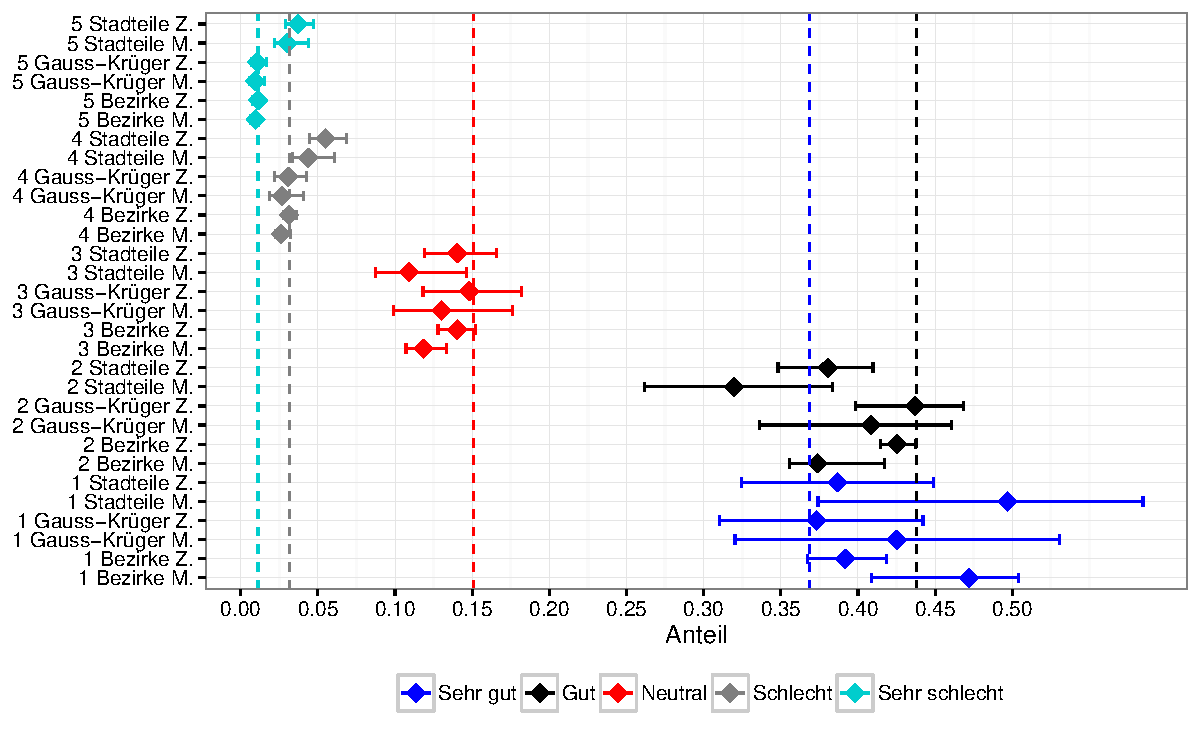
\includegraphics[scale=0.8]{Pictures/WohngegendAlleModelle2}
 \caption{Vergleich der extrapolierten Gesamtanteile für Stuttgart mit allen geschätzten Modellen und beiden Extrapolationsdateien mit den Anteilen der Stichprobe mit 95\% Quantielen zur Bewertung der Wohngegend}
 \label{WAlle}
 \end{center}
\end{figure}

Die Ergebnisse der Extrapolation für die Bewertung der Wohngegend sind aus Abbildung \ref{WAlle} ersichtlich. Sie ist analog zu der  bereits diskutierte Abbildung \ref{S21Alle} aufgebaut, außer dem Unterschied dass keine Anteile für die Grundgesamtheit verfügbar sind. Hier ist gerade bei den Klassen \textit{neutral}, \textit{gut} und \textit{sehr gut} ein deutlicher Unterschied zwischen den Modellen erkennbar, sowohl für den Punkt- als auch den Intervallschätzer. Auch zwischen den Dateien sind wie schon bei der Meinung zu Stuttgart 21 deutliche Unterscheide vorhanden. Um in dieser Arbeit konsistent zu bleiben und da der Melderegister mehr Beobachtungen hat, folgt die weitere Analyse wieder mit diesem. Die Prognoseintervalle unterscheiden sich relativ stark zwischen den Modellen und den Klassen. Die schmalsten Prognoseintervalle liefert das Bezirkmodell, während das Gauß-Krüger- und Stadtteilmodell deutlich weitere Intervalle ergibt. Aggregiert auf Bezirksebene ergeben sich für die Klasse \textit{sehr gut} 42,52\% für das Gauß-Krüger Modell, 47,18\% für das Bezirkmodell und 49,71 \% für das Stadtteilmodell.  Für die Klasse \textit{gut} wurden 40,84\% für das Gauß-Krüger Modell, 37,37\% für das Bezirkmodell und 31,98 \% für das Stadtteilmodell prognostiziert. Die Klasse \textit{neutral} wurde von den Modellen in bisheriger Reihenfolge mit 13,08\%, 11,86\% und 10,91\% ermittelt. Die prognostizierten Anteile der Personen mit der Meinung \textit{schlecht}  sind 2,68\%, 2,61\% und 4,37\% . Die letzte Klasse \textit{sehr schlecht} wurde mit 0,95\%, 0,97\% und 3,03\% vorhergesagt. Es ist dabei ein deutlich größerer Unterschied zu beobachten als bei den geschätzten Anteilen der Meinung zu Stuttgart 21, wodurch die Wahl des finalen Prognosemodells noch zusätzliche Wichtigkeit bekommt. Wie bereits erwähnt, kann nur spekuliert werden, wo die wahren Anteile zur Bewertung der Wohngegend liegen. Dadurch stehen auch nur die drei Kriterien AIC, Reklassifizierung und Kreuvalidierung nur Verfügung. Nach diesen Kriterien wird auch für diesen Fall das Modell mit den Gauß-Krüger Informationen als bestes Prognosemodell empfohlen, da es in allen drei Situationen die besten Ergebnisse gezeigt hat.\\
Zuletzt wurden die beiden besten Modelle genutzt um die Extrapolierten Anteile auf Stadtteileebene in Stuttgart darzustellen. Die beiden Abbildungen dazu befinden sich im Anhang. Für die Meinung zu Stuttgart 21 (Abbildung \ref{S21Extra}) kann dazu gut ein Vergleich mit den Anteile der Stichprobe aus Abbildung \ref{XYStuttgart3}, Abbildung \ref{BStuttgart21} und Abbildung \ref{SStuttgart21} vorgenommen werden. Dabei zu beachten ist, dass Abbildung \ref{S21Extra} mit unterschiedlicher Skalierung dargestellt wird, um deutlicher räumliche Unterschiede innerhalb der Klassen zu erkennen. Deutlich zu erkennen, ist dass die Lokalisierung der Anteile in den Kategorien sehr ähnlich ist zu der bereits besprochenen Lokalisierung im Parametrisierungsdatensatz ist. Die hohen Anteile der \textit{Zustimmung} befinden sich vor allem im Norden und Osten, die Klasse \textit{neutral} zeigt keine klare Struktur und die Klasse \textit{Ablehnung} findet sich besonders im Süden und Westen.\\
Auch für die Bewertung der Wohngegend (Abbildung \ref{WohnExtra}) lässt sich ebenfalls ein guter Vergleich mit den Anteilen des Parametrisierungsdatensatz (Abbildung \ref{XYWohnG5}, Abbildung \ref{BWohn}, Abbildung \ref{SWohn}) vorgenommen werden. Besonders interessant sind hier die Kategorien \textit{neutral}, \textit{schlecht} und \textit{sehr schlecht}. Aus Abbildung \ref{BWohn} geht z.B hervor, dass die höchsten Anteile dieser Klassen im Osten und teilweise im Norden lokalisiert werden können. Durch die Extrapolation konnten wir den Bereich nun genauer isolieren auf und um das Benzviertel herum. Hier scheinen die Bewohner Stuttgarts im Vergleich zum Rest der Stadt eher unzufrieden mit ihrer Wohngegend zu sein


\clearpage
\section{Diskussion}
Die beiden Datensätze zur Grundgesamtheit stammen aus einer Melderegister mit 470.190 Beobachtungen und dem Zensus mit 380.238 Beobachtungen. Im Verhältnis zu den Grundgesamtheiten dieser Größenordnung sind 3143 Beobachtungen in der Stichprobe relativ gering, was eine gewisse Unsicherheit für die Extrapolation mit sich bringt [...].\\
Weiterhin ist zu beachten, dass Informationen zu dem monatlichen Netto Haushaltseinkommen in beiden Grundgesamtheiten fehlen und somit die Variable nicht für die Prognose verwendet werden kann. Auch war eine denkbare Erstellung von Proxy-Variablen nicht möglich. Eine genaue Auflistung der enthaltenen Variablen aus den Grundgesamtheiten ist im Anhang verfügbar. Die Arbeit zielt darauf ab, die Meinung der Befragten zu dem Projekt Stuttgart 21 und die Zufriedenheit mit der Wohngegend der Befragten auf die Grundgesamtheit zu extrapolieren. Daher ist es sinnvoll die Ausprägungen dieser Variablen genauer zu untersuchen.\\

\textcolor{red}{In Benzviertel und Wasen gibt es keine einzige Beob. im Param. D aber in beiden extrap. D. Hier ist die Wohnz. schlechter als umzu}\\
Insgesamt ist zu sagen, dass die Gauß-Krüger Informationen ein relativ klaren Einblick in die Verteilung der Beobachtungen in der jeweiligen Klasse geben. Bei den diskreten räumlichen Informationen könnte die grobe Aufteilung auf Bezirksebene zu einem Underfitting und die sehr feine Aufteilung auf Stadtteilebene zu einem Overfitting führen [...]. Zudem ist zu vermuten, dass die räumlichen Informationen einen stärkeren Effekt auf die Bewertung der Wohngegend haben, als auf die Meinung zu Stuttgart 21.

Ein \textit{B} von 1.000 erwies sich als ausreichend, da sich die Mittelwerte und Quantile bei einer Erhöhung kaum noch änderten.

modelle: Frauen eher ablehnen deutete sich an: internet service stuttgart

%============================================== Conlcusion =========================================================%

\section{Fazit}

\clearpage


%============================================ References ===========================================================%
\addcontentsline{toc}{section}{\numberline{}Literatur}
\bibliographystyle{apalike}
\bibliography{LiteraturStuttgart.bib} 

%\section{References}
%\renewcommand{\section}[2]{}
%\addcontentsline{toc}{section}{References}
%\renewcommand{\bibname}{4 References}
%\phantomsection
%\addcontentsline{toc}{section}{References}




\clearpage

%============================================== Appendix ============================================================%
%\appendix
%\pagestyle{Myheadings}
\chead{ANHANG}
%\pagestyle{}
%\section{$A^{-1}$ Appendix}
%\setcounter{secnumdepth}{0}

\begin{appendix}

\section*{Anhang}
\addcontentsline{toc}{section}{\numberline{}Anhang}






\begin{figure}[h]
 \begin{center}
 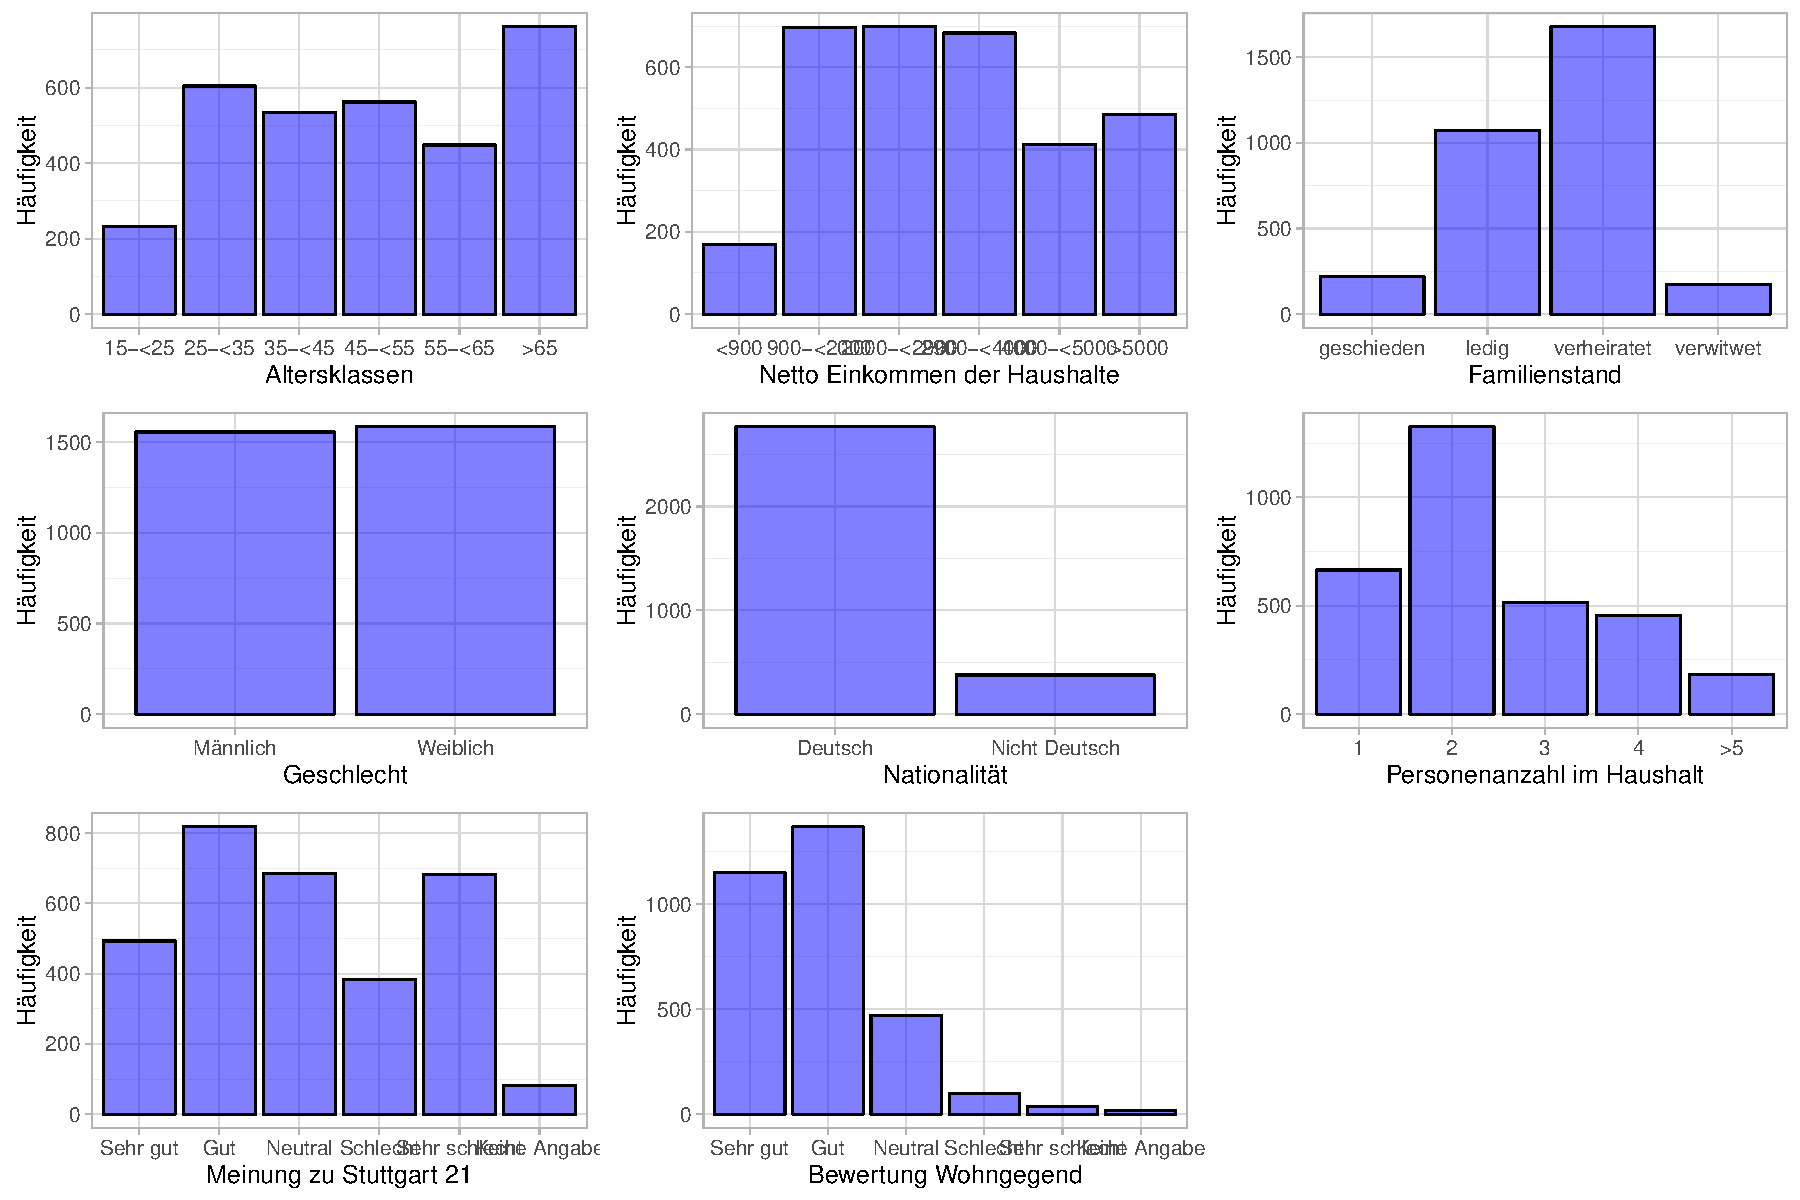
\includegraphics[scale=0.8]{Pictures/BarData}
 \caption{Häufigkeit der Kategorienausprägungen der exogenen Variablen in der Parameterisierungsstichprobe.}
 \label{exogen_parametrisierungsdatensatz}
 \end{center}
\end{figure}


\begin{figure}[h]
 \begin{center}
 
\includegraphics[scale=0.8]{Pictures/BWohn}
 \caption{Anteile der Bewertung der Wohngegend nach Stadtbezirken.}
 \label{BWohn}
 \end{center}
\end{figure}

\begin{figure}[h]
 \begin{center}
 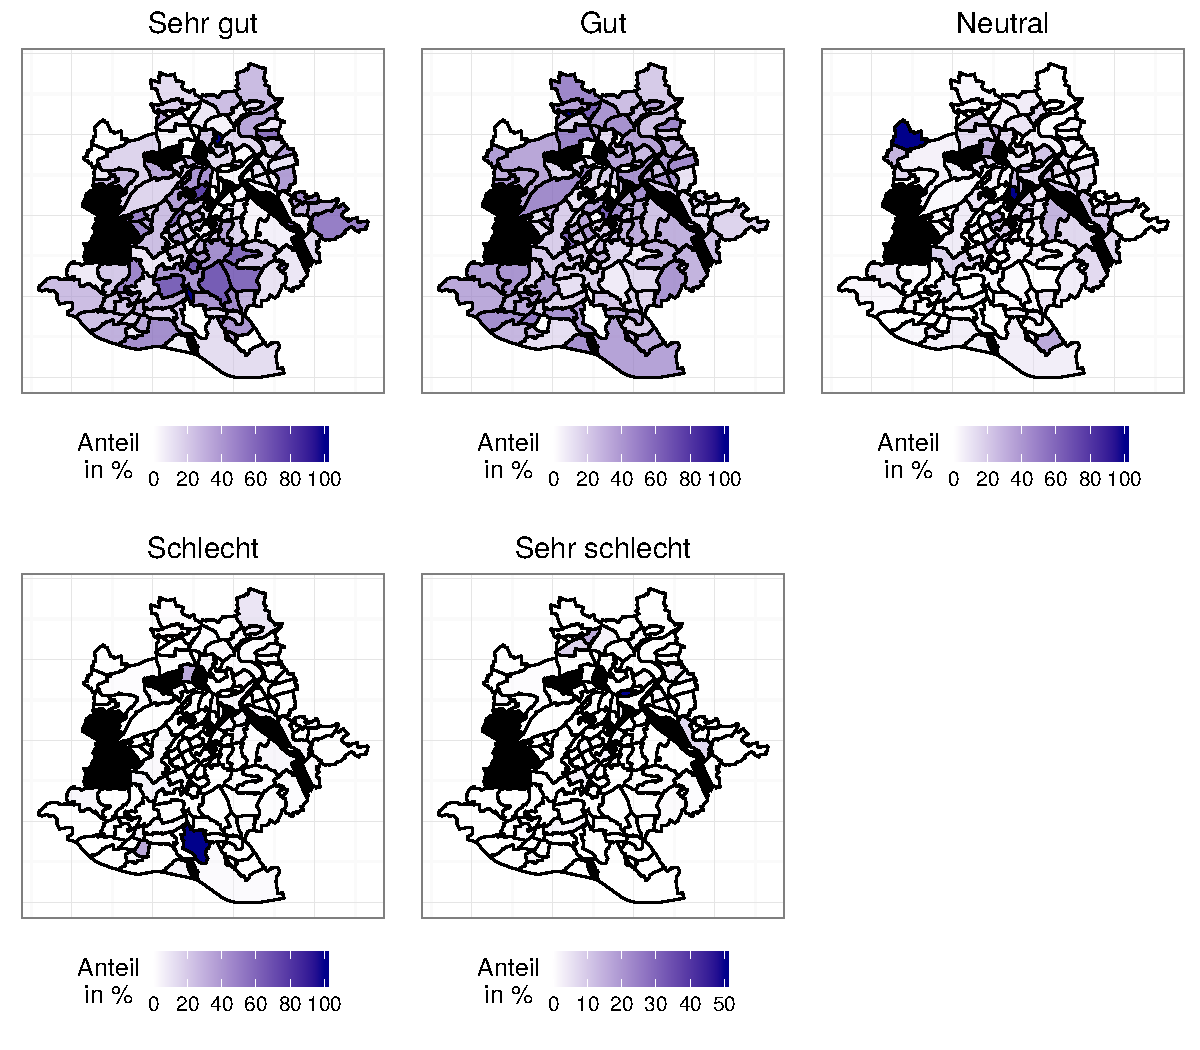
\includegraphics[scale=0.8]{Pictures/SWohn}
 \caption{Anteile der Bewertung der Wohngegend nach Stadtteilen.}
 \label{SWohn}
 \end{center}
\end{figure}

%\begin{figure}[h]
% \begin{center}
% 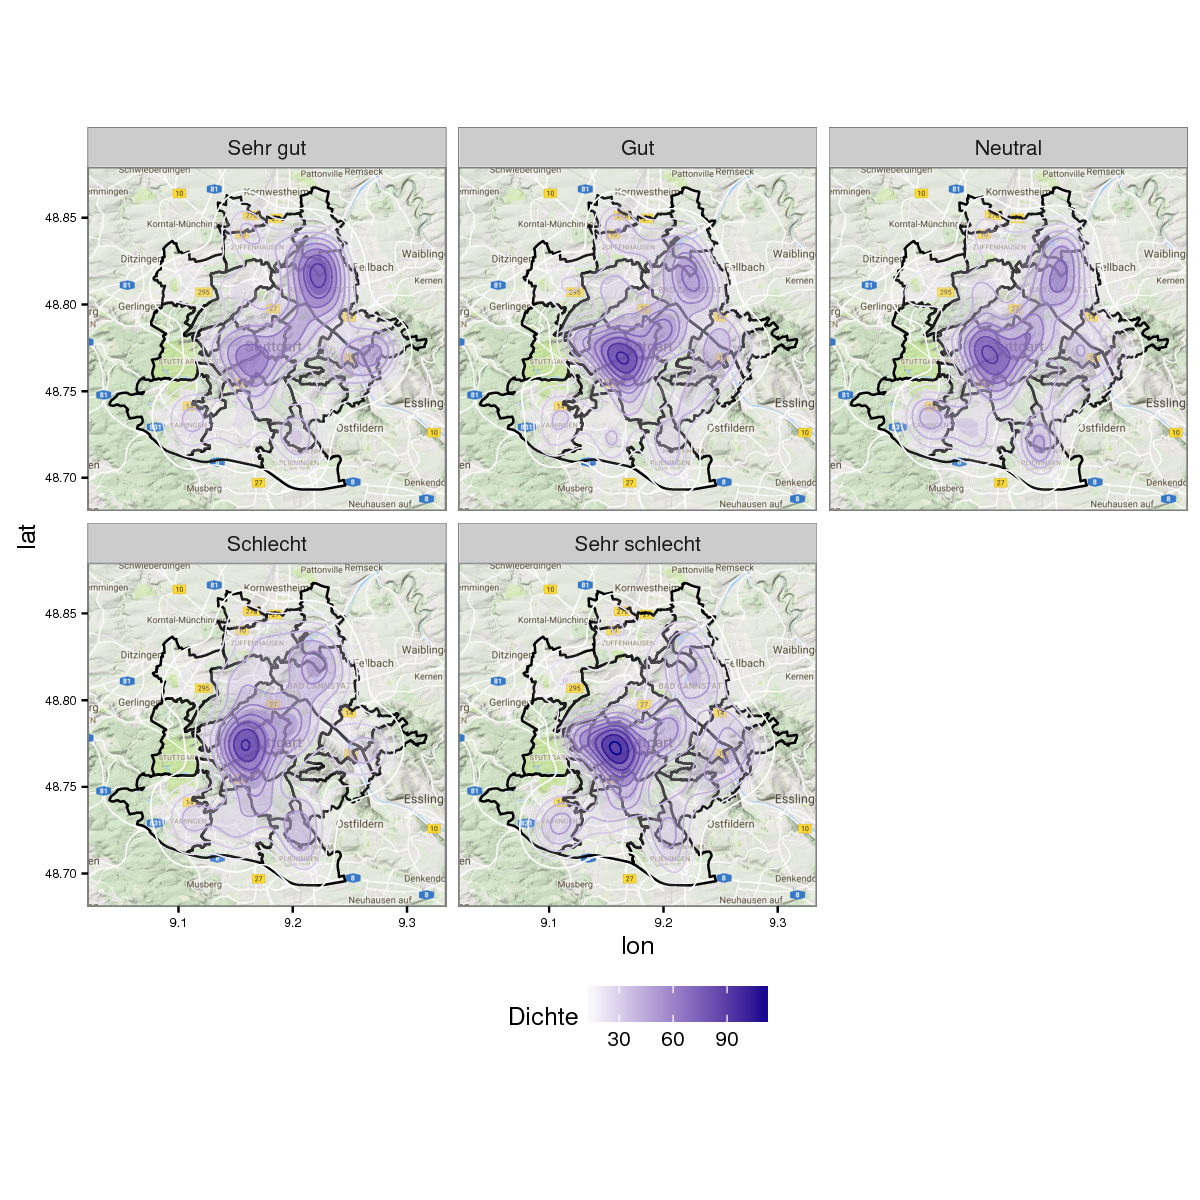
\includegraphics[scale=0.8]{Pictures/XYStuttgart5}
% \caption{Gauß Krüger Informationen Stuttgart 21 (2)}
% \label{endogene}
% \end{center}
%\end{figure}

\begin{figure}[h]
 \begin{center}
 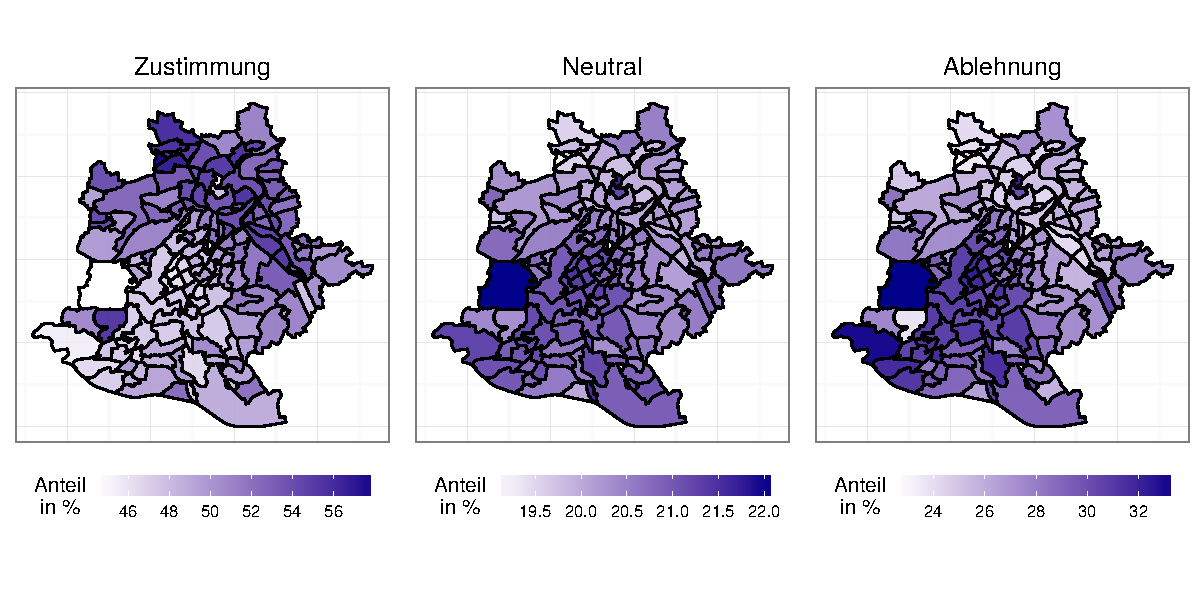
\includegraphics[scale=0.8]{Pictures/S21Extra}
 \caption{Extrapolierte Anteile auf Stadtteilebene für die Meinung zu Stuttgart 21 mit dem besten Modell}
 \label{S21Extra}
 \end{center}
\end{figure}

\begin{figure}[h]
 \begin{center}
 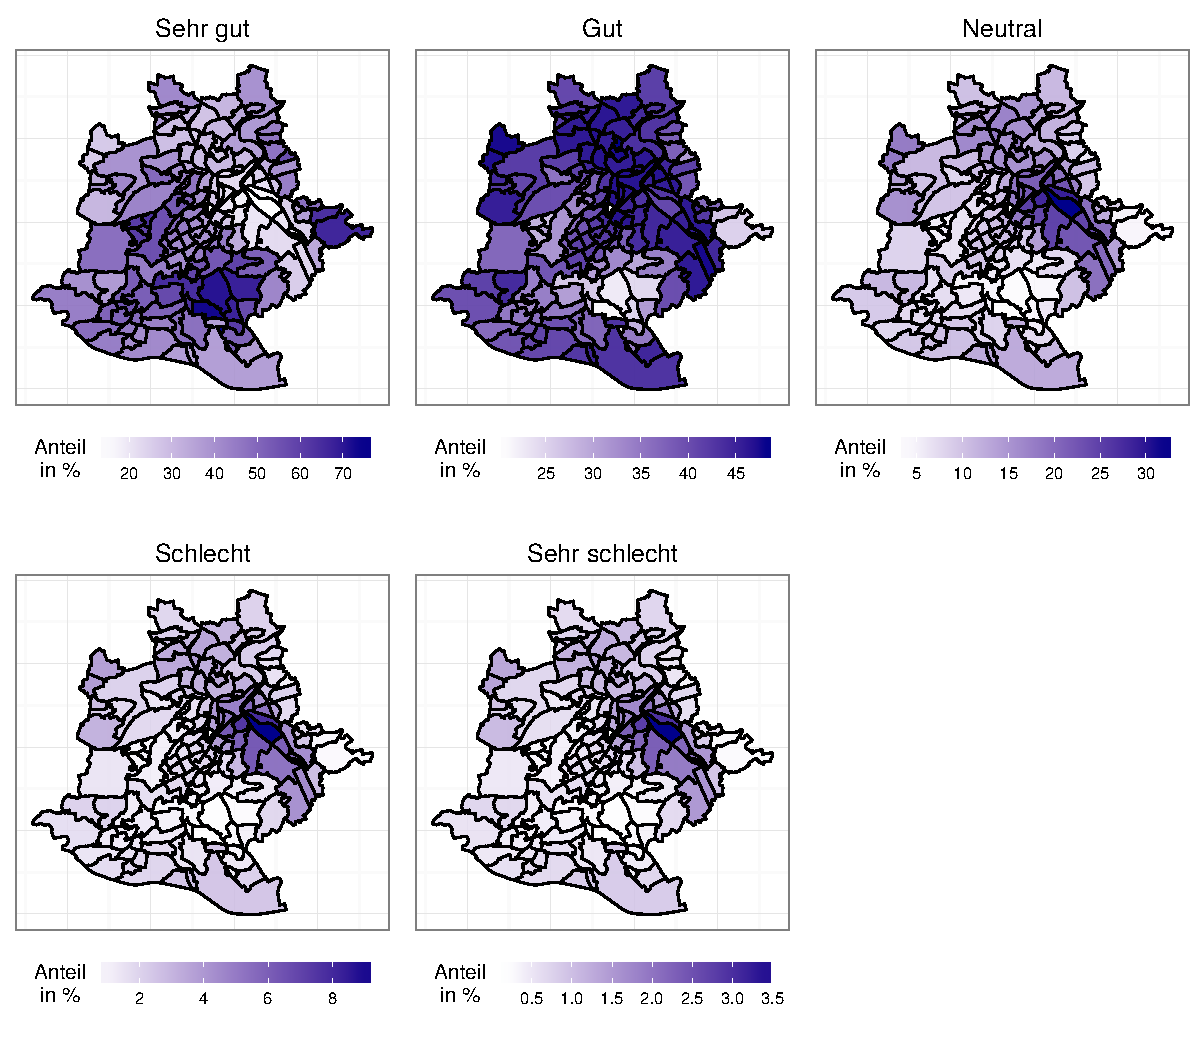
\includegraphics[scale=0.8]{Pictures/BWohnExtra}
 \caption{Extrapolierte Anteile auf Stadtteilebene für die Bewertung der Wohngegend mit dem besten Modell}
 \label{WohnExtra}
 \end{center}
\end{figure}

\end{appendix}
\clearpage
\pagestyle{plain}
%\phantomsection
%\addcontentsline{toc}{section}{Eigenständigkeitserklärung}

%\section{Eigenständigkeitserklärung}

Hiermit versichere ich, dass ich die vorliegende Hausarbeit selbstständig verfasst und keine anderen als die angegebenen
Hilfsmittel benutzt habe. Alle wörtlich oder sinngemäß den Schriften anderer entnommenen Stellen
habe ich unter Angabe der Quellen kenntlich gemacht. Dies gilt auch für beigefügte Zeichnungen, Skizzen, bildliche
Darstellungen und dergleichen.\\
\\
Mir ist bewusst, dass ich mich im Falle einer unbeabsichtigten oder vorsätzlichen Missachtung durch den fehlerhaften
Umgang mit Quellen unter Umständen strafbar mache und die vorliegende Hausarbeit mit nicht ausreichend
bewertet wird.
\\
\\Göttingen, den
\\Unterschrift
\vspace*{4cm}
\\
Hiermit erlaube ich, dass meine Arbeit auf Betrug und falsche, sowie fehlende Zitate auch online geprüft wird.\\
\\
Mir ist bewusst, dass ich mich im Falle einer unbeabsichtigten oder vorsätzlichen Missachtung durch den fehlerhaften
Umgang mit Quellen unter Umständen strafbar mache und die vorliegende Hausarbeit mit nicht ausreichend
bewertet wird.
\\
\\Göttingen, den
\\Unterschrift
\clearpage


\end{document}
